% XeLaTeX can use any Mac OS X font. See the setromanfont command below.
% Input to XeLaTeX is full Unicode, so Unicode characters can be typed directly into the source.

% The next lines tell TeXShop to typeset with xelatex, and to open and save the source with Unicode encoding.

%!TEX TS-program = xelatex
%!TEX encoding = UTF-8 Unicode

\documentclass[12pt, twoside]{book}
\usepackage[bottom=1.25in]{geometry}                % See geometry.pdf to learn the layout options. There are lots.
\geometry{a4paper}                   % ... or a4paper or a5paper or ... ....
%\geometry{landscape}                % Activate for for rotated page geometry
\usepackage[parfill]{parskip}    % Activate to begin paragraphs with an empty line rather than an indent
\usepackage{graphicx}
\usepackage{amssymb}
\usepackage{float}
\usepackage{pgfornament}
\usepackage{multirow}
\usepackage{lscape}
\usepackage{pdfpages}
\usepackage{emptypage}
\usepackage{fontspec,xltxtra,xunicode}
%\defaultfontfeatures{Mapping=tex-text}
\setromanfont[Mapping=tex-text]{Hoefler Text}
\setsansfont[Scale=MatchLowercase,Mapping=tex-text]{Gill Sans}
\setmonofont[Scale=MatchLowercase]{Andale Mono}

\usepackage{polyglossia}
\XeTeXlinebreaklocale "th"
\XeTeXlinebreakskip = 0pt plus 1pt %
\defaultfontfeatures{Scale=1.23}
\setdefaultlanguage{thai}
%\newfontfamily{\thaifont}{TH SarabunPSK}
\newfontfamily{\thaifont}{TH Sarabun New}

% Thai Sarabun font declaration and settings
\fontspec[				
ItalicFont={TH Sarabun New Italic},
BoldFont={TH Sarabun New Bold},
BoldItalicFont={TH Sarabun New Bold Italic},
]{TH Sarabun New}

\title{คู่มือสนามบินส่วนบุคคล \\
	สนามบินขนงพระ \\
	Private Aerodrome Manual \\
	Khanong Phra Airport (KNP) \\
}

\author{ \pgfornament[color=red!40!black, width=5cm]{88} \\
			\LARGE{อนุทิน ชาญวีรกูล}  \\
			\pgfornament[color=red!40!black, width=5cm]{88} \\ \\ \\
}
			
\date{\Large{สิงหาคม 2561}}    % Activate to display a given date or no date

\begin{document}

\maketitle				% Cover page
\newpage\mbox{}\thispagestyle{empty}\newpage
\pagenumbering{roman} 	% Use Roman page numbering
%!TEX TS-program = xelatex
%!TEX encoding = UTF-8 Unicode

\chapter*{คำนำ}

%คู่มือสนามบินส่วนบุคคล
%สนามบินขนงพระ
%Private Aerodrome Manual
%Kanong Phra Airport

คู่มือสนามบินส่วนบุคคลเป็นข้อกำหนดพื้นฐานของกระบวนการออกใบอนุญาตจัดตั้งสนามบินส่วนบุคล คู่มือจะมีข้อมูลทั้งปวงเกี่ยวข้องโดยตรงกับสถานที่ตั้ง สิ่งอำนวยความสะดวก วิธีดำเนินการ การจัดการความปลอดภัยด้วย ข้อมูลที่ปรากฏอยู่ในคู่มือสนามบินแสดงให้เห็นว่าสนามบินมีความปลอดภัยสำหรับการปฏิบัติการเป็นสนามบินส่วนบุคค  และแสดงให้เห็นว่าไม่มีข้อบกพร่องที่เด่นชัดซึ่งจะมีผลกระทบในทางเสียหายต่อความปลอดภัยของการปฏิบัติการอากาศยาน 

คู่มือนี้เป็นเอกสารอ้างอิงและเป็นรายการตรวจสอบการคงไว้ซึ่งมาตรฐานการจัดตั้งสนามบินส่วนบุคคล ข้อมูลที่อยู่ในคู่มือสนามบินส่วนบุคคลนี้จะช่วยให้สำนักงานการบินพลเรือนแห่งประเทศไทย (กพท.) ประเมินความเหมาะสมของสนามบินสำหรับการปฏิบัติการอากาศยานที่ยื่นเสนอมา คู่มือนี้เป็นแนวทางอ้างอิงพื้นฐานสำหรับทำการตรวจพินิจสถานที่ในสนามบินและเพื่อการตรวจพินิจความปลอดภัยในเวลาต่อมา คู่มือสนามบินนี้เป็นเอกสารอ้างอิงที่ยอมรับระหว่างสนามบินบ้านธิ และสำนักงานการบินพลเรือนแห่งประเทศไทยในเรื่องของมาตรฐาน เงื่อนไข และระดับการให้บริการซึ่งต้องคงไว้ที่สนามบิน \\
\vskip 10pt


อนุทิน ชาญวีรกูล \\
สนามบินขนงพระ \\
\date{สิงหาคม 2561} \\

%!TEX TS-program = xelatex
%!TEX encoding = UTF-8 Unicode

\chapter*{รายการปรับปรุงแก้ไขคู่มือสนามบินส่วนบุคคลขนงพระ (List of Effective Pages)}

\begin{table}[h!]
\caption{รายการ การปรับปรุงแก้ไขคู่มือสนามบินส่วนบุคคลขนงพระ}
\begin{center}
\begin{tabular}{|c|c|c|c|c|}
\hline
\textbf{ครั้งที่} & \textbf{หน้าที่มีการเปลี่ยนแปลง} & \textbf{วันที่มีผลใช้งาน} & \textbf{วันที่บรรจุในคู่มือ} & \textbf{ผู้ที่ดำเนินการบรรจุลงในคู่มือ} \\
\textbf{No} & \textbf{Affected Pages} & \textbf{Date Applicable} & \textbf{Date Entered} & \textbf{Entered by} \\ \hline
 Original & ทุกหน้า & สิงหาคม 2561 & สิงหาคม 2561 & อนุทิน ชาญวีรกูล \\ \hline
 & & & & \\ \hline
 & & & & \\ \hline
 & & & & \\ \hline
 & & & & \\ \hline
 & & & & \\ \hline
 & & & & \\ \hline
 && & & \\ \hline
 & & & & \\ \hline
 & & & & \\ \hline
 & & & & \\ \hline
 & & & & \\ \hline
 & & & & \\ \hline
 & & & & \\ \hline
 & & & & \\ \hline
 & & & & \\ \hline
 & & & & \\ \hline
 & & & & \\ \hline
& & & & \\ \hline
 & & & & \\ \hline
 & & & & \\ \hline
\end{tabular}
\end{center}
\label{รายการ การปรับปรุงแก้ไขคู่มือสนามบินส่วนบุคคลขนงพระ}
\end{table}%

\tableofcontents		% Table of Contents
\listoftables			% List of Tables
\listoffigures			% List of Figures
\newpage\mbox{}\thispagestyle{empty}\newpage
\clearpage				% Clear Roman page numbering
\pagenumbering{arabic} 	%Use Arabic page numbering for contents

%!TEX TS-program = xelatex
%!TEX encoding = UTF-8 Unicode

\chapter{ข้อมูลทั่วไป \\
General Information}

\section{วัตถุประสงค์และขอบเขตของคู่มือสนามบิน}

คู่มือปฏิบัติงานสนามบินฉบับนี้ มีจุดประสงค์ดังนี้
	\begin{enumerate}
	\item เพื่อใช้แสดงถึงวิธีปฏิบัติงานของสนามบินให้เกิดความปลอดภัยต่ออากาศยาน
	\item เพื่อใช้เป็นที่รวบรวมข้อมูลสนามบิน
	\item เพื่อใช้เป็นเอกสารอ้างอิงสำหรับการตรวจสอบการดำเนินงานสนามบินให้เป็นไปตามข้อกำหนดและมาตรฐานต่าง ๆ
\end{enumerate}

คู่มือฯนี้มีขอบเขต ดังนี้
วิธีการปฏิบัติงานสำหรับสนามบินขนงพระ เพื่อความปลอดภัยของอากาศยานที่ปฏิบัติการบินที่สนามบินขนงพระ เท่านั้น

\section{ข้อกฎหมายที่เกี่ยวข้องกับการขอและออกใบอนุญาตสนามบินส่วนบุคคล }

\begin{enumerate}
	\item พระราชบัญญัติการเดินอากาศ พ.ศ. 2497 ซึ่งแก้ไขเพิ่มเติมโดย พระราชบัญญัติการเดินอากาศ (ฉบับที่ 11) พ.ศ. 2551
	\item กฎกระทรวงว่าด้วยการขอและการออกใบอนุญาตจัดตั้งสนามบิน พ.ศ. 2550
	\item ประกาศสำนักงานการบินพลเรือนแห่งประเทศไทยเรื่องมาตรฐานคู่มือสนามบินส่วนบุคคล พ.ศ. 2561
\end{enumerate}

\section{เงื่อนไขการอนุญาตใช้สนามบิน (Conditions of Use)}

\subsection{รายละเอียดแสดงช่วงเวลาทำงานของสนามบินส่วนบุคคล}

สนามบินขนงพระ มีช่วงเวลาทำงานตั้งแต่เวลาประมาณ 6:00 น. ถึง 18:00 น. และมีช่วงเวลาเปิดใช้บริการแก่อากาศยานตั้งแต่พระอาทิตย์ขึ้น ถึง พระอาทิตย์ตก และเวลาอื่นนอกเหนือจากนี้โดยเปิดให้ใช้เป็นกรณีไปตามที่ร้องขอ  การนำอากาศยานมาขึ้นลงจะต้องได้รับอนุญาตจากผู้จัดการสนามบินหรือผู้ได้รับมอบหมายก่อนทุกครั้ง เนื่องจากเป็นสนามบินส่วนบุคคล \\
	
\noindent หมายเลขโทรศัพท์ติดต่อผู้จัดการสนามบิน 086 657 1510 

\subsection{รายละเอียดประประเภทของกฎการจราจรที่ต้องปฏิบัติ}

กฎการบินทั่วไป (GENERAL RULES) และ กฎการบินด้วยทัศนวิสัย (VFR)

\subsection{รายละเอียดประประเภททางวิ่งที่ให้บริการ}

ทางวิ่ง 10 ประเภท Non – Instrument Runway \\
ทางวิ่ง 28 ประเภท Non –Instrument Runway 

\subsection{รายละเอียดที่แสดงว่าสนามบินส่วนบุคคลไม่ได้ปิดให้บริการแก่บุคคลภายนอก}

\begin{enumerate}
	\item สนามบินขนงพระได้รับใบอนุญาตจัดตั้งเป็นสนามบินส่วนบุคคล และตามเงื่อนไขใบอนุญาต และวิธีปฏิบัติการของสนามบินขนงพระให้ใช้งานเป็นแบบสนามบินส่วนบุคคล
	\item รายละเอียดใบอนุญาตจัดตั้งเป็นสนามบินส่วนบุคคล  ตามแสดงในคู่มือฯนี้ \footnote{รายละเอียดในภาคผนวก ก. (\ref{ใบอนุญาตที่ขึ้นลงชั่วคราวอากาศยานขนงพระ})}
	 
\end{enumerate}

\subsection{ระบบการบันทึกข้อมูลของอากาศยาน (Recordings 0f Aircraft Movements) ที่แสดงถึงเที่ยวบินขาเข้าและขาออก}

\begin{enumerate}
	\item ก่อนทำการบินทุกครั้ง ผู้ทำการบินจะต้องยื่นแผนการบิน ( Flight Plan ) ไปยังหน่วยงานให้บริการจราจรทางอากาศตามรูปแบบของแผนการบิน ได้แก่ ข้อมูลของอากาศยานที่จะทำการบินมา ณ สนามบินขนงพระ ประกอบด้วย ชื่อนักบิน แบบอากาศยาน เครื่องหมาย สัญชาติ และทะเบียน เวลามาถึง/ออกจากสนามบิน
	\item ข้อมูลสถิติเที่ยวบินขาเข้าและขาออก  จะลงบันทึกในสมุดปูมของสนามบิน (Airfield Log) โดยมี รายละเอียดเกี่ยวกับเที่ยวบิน ประกอบด้วย ชื่อนักบิน แบบอากาศยาน เครื่องหมาย สัญชาติ และทะเบียน เวลามาถึง/ออกจากสนามบิน 
\end{enumerate}

\subsection{กรณีมีเที่ยวบินทำการบิน ณ สนามบินขนงพระ โดยไม่ได้รับอนุญาต}

ในกรณีที่พบว่ามีเที่ยวบินที่ไม่ได้รับอนุญาตทำการบิน ณ สนามบินขนงพระ โดยไม่ใช่เที่ยวบินที่มีเหตุจำเป็นฉุกเฉิน เจ้าหน้าที่จะรายงานข้อมูลเที่ยวบิน เช่น เครื่องหมายทะเบียน แบบอากาศยาน และชื่อนักบิน ไปยังสำนักงานการบินพลเรือนแห่งประเทศไทย

ระบบการบันทึกข้อมูลของอากาศยาน (Recordings 0f Aircraft Movements) ที่แสดงถึงเที่ยวบินขาเข้า

\section{หน้าที่และความรับผิดชอบของผู้ได้รับใบอนุญาตจัดตั้งเป็นสนามบินส่วนบุคคล (Private Aerodrome Operator)}

\begin{enumerate}
	\item ตามกฎกระทรวง การว่าด้วยการขอและการออกใบอนุญาตจัดตั้งสนามบิน พ.ศ. 2550  ผู้ขอจัดตั้งต้องมีความรู้ความสามารถในการจัดการสนามบินส่วนบุคคลตามที่อธิบดีประกาศกำหนด \\

	นายอนุทิน ชาญวีรกูล ได้รับอนุญาตให้จัดตั้งที่ขึ้นลงชั่วคราวของอากาศยานครั้งแรกตามใบอนุญาตเลขที่ 1535/2556 เมื่อวันที่ 17 ธันวาคม 2556 และได้รับการต่ออายุมาโดยตลอด รวมระยะเวลามากกว่า 4 ปี โดยครั้งล่าสุด ได้รับใบอนุญาตจัดตั้งฯ ที่ 654/2559 และ นายอนุทิน ชาญวีรกูล ได้ดำเนินการที่ขึ้นลงชั่วคราวฯ อย่างปลอดภัยมาโดยตลอด รวมทั้งปฏิบัติตามคำสั่งของทางราชการอย่างเคร่งครัด   จึงแสดงให้เห็นถึงว่า นายอนุทิน ชาญวีรกูล มีความรู้ความสามารถในการจัดการสนามบินส่วนบุคคล เป็นอย่างดี
	\item ตามประกาศสำนักงานการบินพลเรือนแห่งประเทศไทยเรื่องมาตรฐานคู่มือสนามบินส่วนบุคคล พ.ศ. 2561 \\
	นายอนุทิน ชาญวีรกูล ในฐานะเจ้าของสนามบินได้ดำเนินการและจักดำเนินการ ดังต่อไปนี้
	\begin{itemize}
		\item ได้จัดทำคู่มือสนามบินส่วนบุคคลตามประกาศฯ และยื่นต่อ สำนักงานการบิน
พลเรือนแห่งประเทศไทย ด้วยคู่มือฯ ฉบับนี้
		\item ปรับปรุงคู่มือฯ ให้มีข้อมูลเป็นปัจจุบัน เสมอ
		\item จัดทำรายละเอียดและแผนปฏิบัติการต่างๆ และปฏิบัติตามรายละเอียดนั้นๆ
		\item จัดหาบุคคลที่มีความรู้ความสามารถมาปฏิบัติงาน
	\end{itemize}
\end{enumerate}

นอกจากนี้ นายอนุทิน ชาญวีรกูล มีหน้าที่และความรับผิดชอบ ตามเงื่อนไขที่ สำนักงานการบินพลเรือนแห่งประเทศไทย จะกำหนดขึ้น และตามกฎหมายอื่นๆที่เกี่ยวข้อง

นายอนุทิน ชาญวีรกูล จะดำเนินงานสนามบินส่วนบุคคล ให้เกิดความปลอดภัยสูงสุด 
				% Chapter 1: Manual General Information 
%!TEX TS-program = xelatex
%!TEX encoding = UTF-8 Unicode

\chapter{ข้อมูลของสถานที่ตั้งสนามบิน \\
Aerodrome Site Details}

\section{แผนผังสนามบินที่แสดงสิ่งอำนวยความสะดวกหลัก}

ประกอบด้วย แผนผังสนามบินและสิ่งอำนวยความสะดวกหลัก และแผนผังอาคารและสิ่งอำนวยความสะดวกภายในสนามบิน ดังแสดงในรูปข้างล่าง

\subsection{แผนผังสนามบินและสิ่งอำนวยความสะดวกหลัก}

\begin{figure}[ht!]
\begin{center}
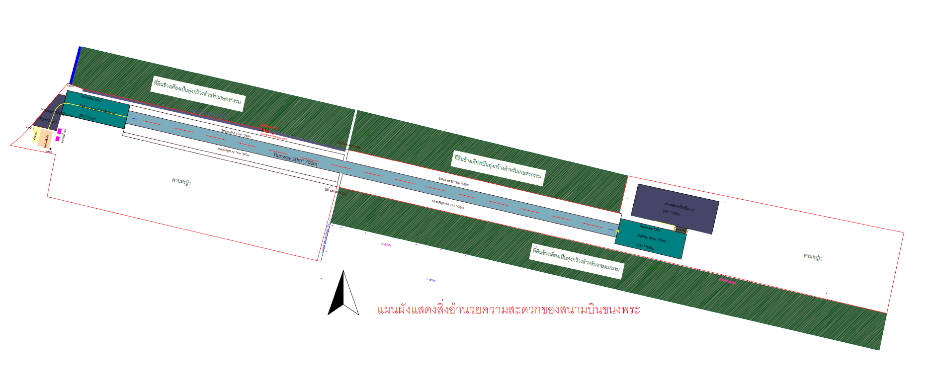
\includegraphics[scale=1.0]{images/Picture1.png}
\caption{แผนผังสนามบินและสิ่งอำนวยความสะดวกหลักของสนามบินขนงพระ}
\label{default}
\end{center}
\end{figure}

\newpage
\subsection{แผนผังแสดงสิ่งอำนวยความสะดวกของสนามบิน}

\begin{figure}[h!]
\begin{center}
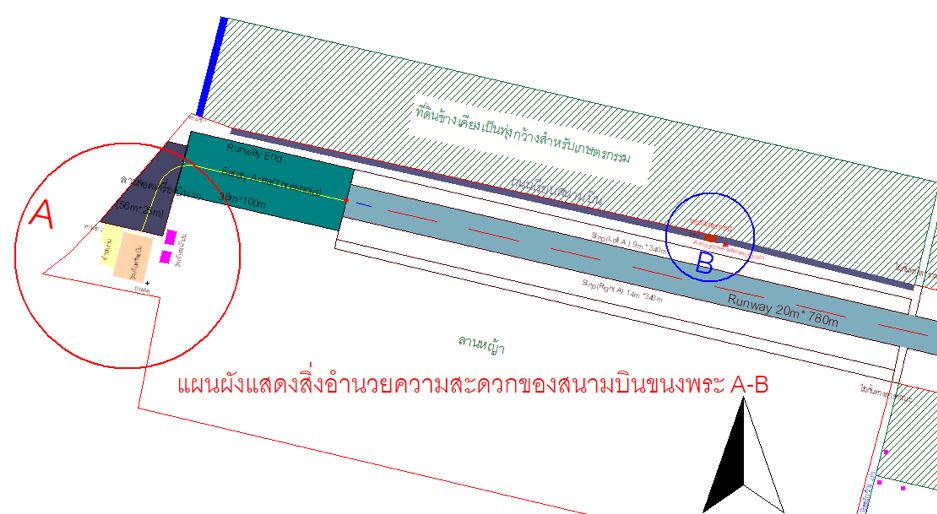
\includegraphics[scale=0.75]{images/Picture2.png}
\caption{แผนผังอาคารและสิ่งอำนวยความสะดวกภายในสนามบิน แสดงส่วยขยาย A และ B}
\label{default}
\end{center}
\end{figure}

\begin{figure}[h!]
\begin{center}
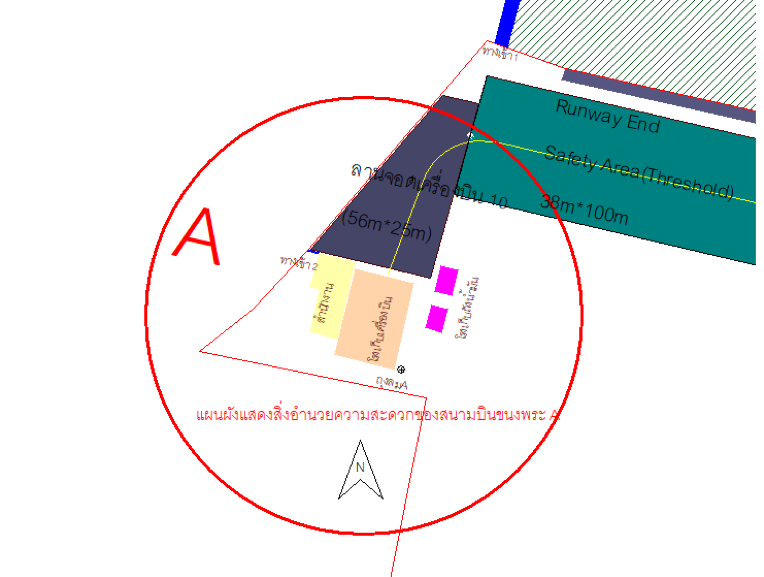
\includegraphics[scale=0.75]{images/Picture3.png}
\caption{แผนผังอาคารและสิ่งอำนวยความสะดวกภายในสนามบิน ขยาย A}
\label{default}
\end{center}
\end{figure}

\begin{figure}[h!]
\begin{center}
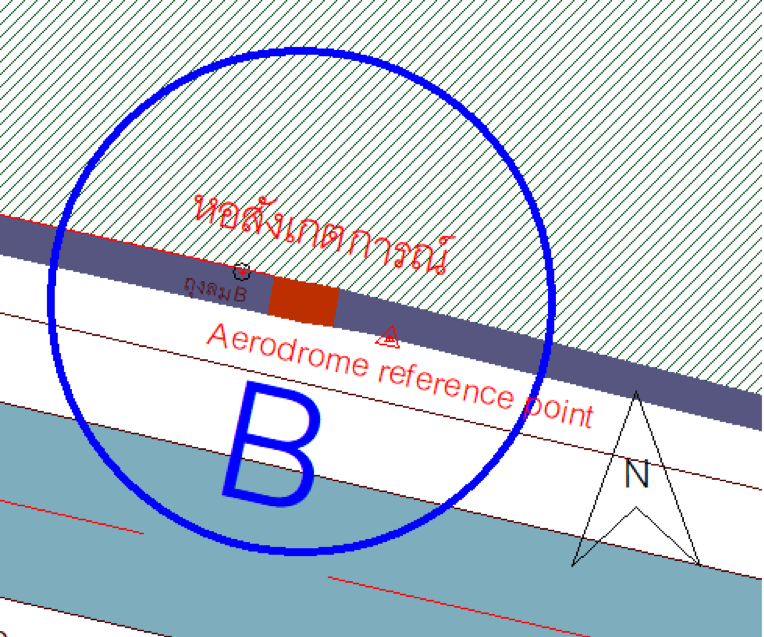
\includegraphics[scale=0.65]{images/Picture4.png}
\caption{แผนผังอาคารและสิ่งอำนวยความสะดวกภายในสนามบิน ขยาย B}
\label{default}
\end{center}
\end{figure}

\section{แผนผังสนามบินแสดงแนวเขตสนามบิน} \label{แผนผังสนามบินแสดงแนวเขตสนามบิน}

สนามบินขนงพระ ตั้งอยู่ในเขตอำเภอปากช่อง จังหวัดนครราชสีมา  ทิศเหนือและทิศตะวันออก เป็นไร่เกษตรกรรม ทิศใต้เป็นไร่ข้าวโพด และป่าไม้ในเขตที่ดินส่วนบุคคล  และทิศตะวันตกเป็นสนามกอล์ฟ  สนามบินมีเนื้อที่ประมาณ 160,050 ตารางเมตร หรือ 100 ไร่ (ดังรูประบายสีฟ้าข้างล่าง)                                      

\begin{figure}[h!]
\begin{center}
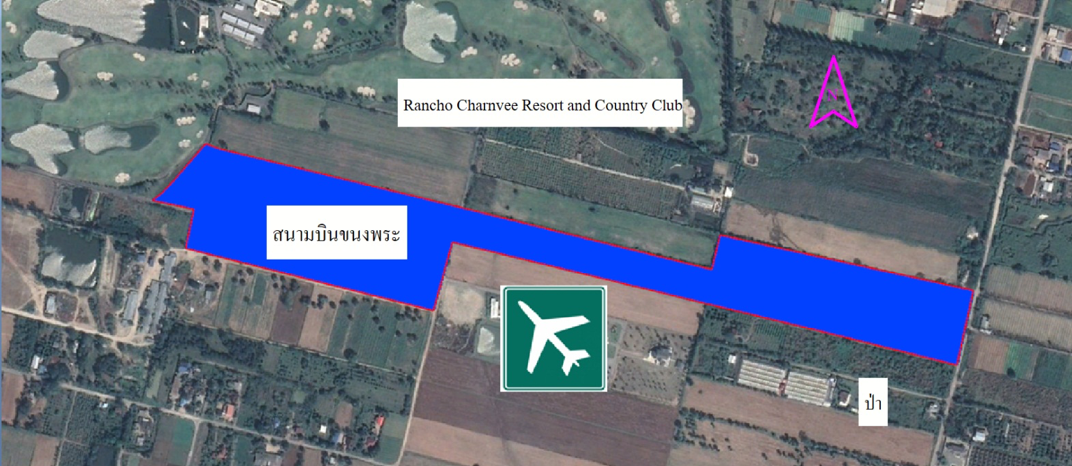
\includegraphics[width=\linewidth]{images/Picture5.png}
\caption{แผนผังแนวเขตสนามบินขนงพระ อำเภอปากช่อง จังหวัดนครราชสีมา}\label{แผนผังแนวเขตสนามบินขนงพระ อำเภอปากช่อง จังหวัดนครราชสีมา}
\label{default}
\end{center}
\end{figure}

\newpage
\section{แผนผังที่แสดงถึงระยะห่างของสนามบินกับเมือง}
	สนามบินขนงพระ ตั้งอยู่ ตำบลขนงพระ อำเภอปากช่อง  จังหวัดนครราชสีมา อยู่ห่างจากตัวอำเภอปากช่อง  15 กิโลเมตร 
\begin{figure}[ht!]
\begin{center}
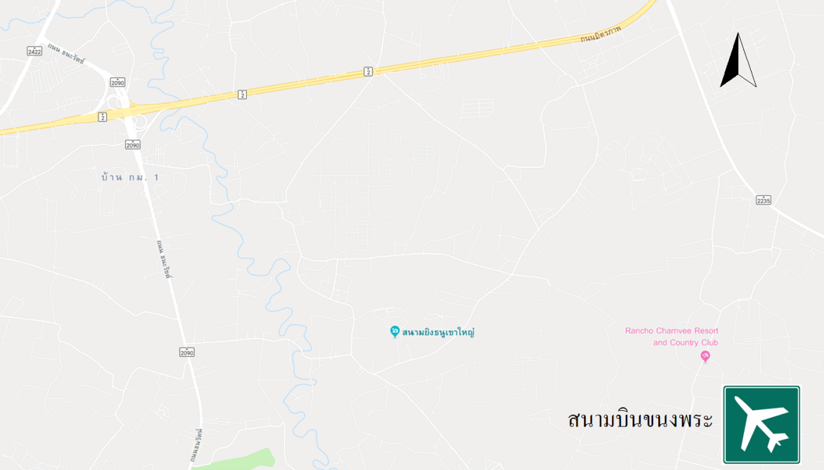
\includegraphics[width=\linewidth]{images/Picture6.png}
\caption{แผนผังแสดงตำแน่งที่ตั้งสนามบินขนงพระ อำเภอปากช่อง  จังหวัดนครราชสีมา}
\label{default}
\end{center}
\end{figure}

\section{หลักฐานแสดงกรรมสิทธิ์ หรือสิทธิครอบครอง หรือสิทธิใช้ประโยชน์ของที่ดิน ที่สนามบินตั้งอยู่}

สถานที่ตั้งสนามบินขนงพระประกอบไปด้วยที่ดิน 7 แปลง รายละเอียดตามภาพและตารางแสดงข้อมูลที่ดิน

\begin{figure}[htbp]
\begin{center}
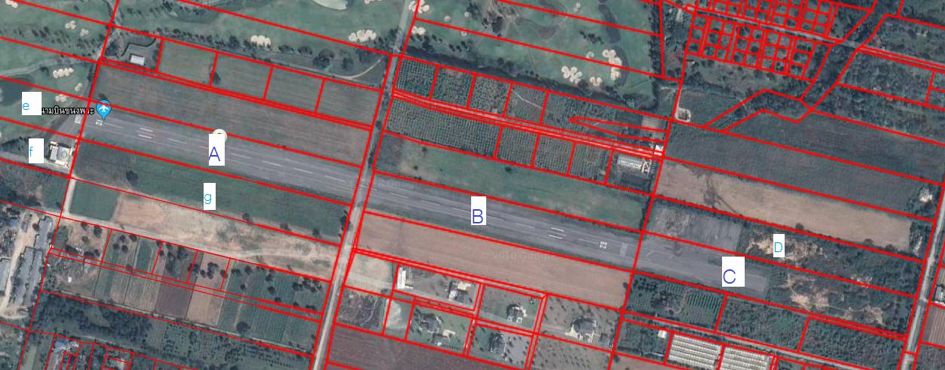
\includegraphics[width=\linewidth]{images/Picture7.png}
\caption{เขตแผนผังโฉนดที่ดินของสนามบินขนงพระ}
\label{default}
\end{center}
\end{figure}

โดยมีรายละเอียดโฉนดที่ดินดังนี้

\begin{enumerate}
\item กรรมสิทธิ์ที่ดินแปลงที่ A B C D และ E เป็นโฉนดที่ดิน และ นส.3 ก ของ บริษัท เจริญคีรี จำกัด โดยนางอนิลรัตน์ นิติสาโรจน์ และนางสาวปราณี พิริยะมาสกุล เป็นกรรมการผู้มีอำนาจลงนาม ได้รับทราบและยินยอมให้นายอนุทิน ชาญวีรกูล เป็นผู้มีอำนาจกระทำการใดๆ ในที่ดินจำนวน 5 แปลงของบริษัทเจริญคีรี จำกัด \footnote{รายละเอียดหนังสือยินยอมจาก บริษัท เจริญคีรี จำกัด ใน ผนวก ข. (\ref{เอกสารสิทธิ์และหนังสือยินยอมให้ใช้ประโยชน์ที่ดินจาก บริษัท เจริญคีรี จำกัด})}
\item กรรมสิทธิ์ที่ดินแปลง F และ G เป็นโฉนดที่ดินของ บริษัท กอล์ฟเขาใหญ่ จำกัด โดยนางอนิลรัตน์ นิติสาโรจน์ และนางสาวปราณี พิริยะมาสกุล เป็นกรรมการผู้มีอำนาจลงนาม ได้รับทราบและยินยอมให้นายอนุทิน ชาญวีรกูล เป็นผู้มีอำนาจกระทำการใดๆ ในที่ดินจำนวน 2 แปลงของบริษัทเจริญคีรี จำกัด \footnote{รายละเอียดหนังสือยินยอมจาก บริษัท กอล์ฟเขาใหญ่ จำกัด ใน ผนวก ข. (\ref{เอกสารสิทธิ์และหนังสือยินยอมให้ใช้ประโยชน์ที่ดินจาก บริษัท กอล์ฟเขาใหญ่ จำกัด})}
\end{enumerate}

\begin{table}[h!]
\caption{รายละเอียดกรรมสิทธิ์ที่ดิน สนามบินส่วนบุคคลขนงพระ}
\begin{center}
\begin{tabular}{|c|c|c|c|c|c|c|} %7 columns
\hline
\multirow{2}{*}{แปลงที่ดิน}  & \multicolumn{5}{c|}{เอกสารสิทธิ์ (โฉนดที่ดิน และ นส. 3ก.)} & \multirow{2}{*}{ผู้ถือกรรมสิทธิ์}  \\ \cline{2-6}
 & เลขที่ & ระวาง & เลขที่ดิน & เล่มที่ & หน้า  &   \\
 \hline
A & โฉนด 41432 & 5238 II 6418 & 166 & 415 & 32 & บริษัท เจริญคีรี จำกัด \\
B & โฉนด 35451 & 5238 II 6618, 6418 & 52 & 355 & 51 & บริษัท เจริญคีรี จำกัด \\
C & โฉนด 35572 & 5238 II 6618 & 191 & 356 & 72 & บริษัท เจริญคีรี จำกัด \\
D & นส.3ก 6322 & -- & 348 & 64ก & 22 & บริษัท เจริญคีรี จำกัด \\
E & นส.3ก 2669 & -- & 167 & 27ข & 19 & บริษัท เจริญคีรี จำกัด \\
F & โฉนด 35445 & 2538 II 6418 & 84 & 355 & 45 & บริษัท กอล์ฟเขาใหญ่ จำกัด \\
G & โฉนด 35446 & 5238 II 6418 & 85 & 355 & 51 & บริษัท กอล์ฟเขาใหญ่ จำกัด \\
\hline 
\end{tabular}
\end{center}
\label{default}
\end{table}%
			% Chapter 2: Aerodrome Site Details
%!TEX TS-program = xelatex
%!TEX encoding = UTF-8 Unicode

\chapter{ข้อมูลสนามบินรายงานต่อฝ่ายข่าวสารการบิน \\
Aerodrome Data for AIS Report}

สนามบินส่วนบุคคล บริเวณขนงพระนี้ เป็น สนามบินสำหรับอากาศยานปีกแข็ง (Fixed-wing Aircraft) 

\section{ข้อมูลทั่วไป (General Information)}

\begin{description}
\item[ชื่อสนามบิน:]  สนามบินขนงพระ
\item[ที่ตั้งสนามบิน:] ตำบลขนงพระ อำเภอปากช่อง จังหวัดนครราชสีมา 30130
\item[ทางภูมิศาสตร์ของจุดอ้างอิงสนามบิน:] Aerodrome Reference Point ที่กำหนดจากฐานอ้างอิงตามระบบ WGS-84 มีรายละเอียดพิกัดและข้อมูล ดังต่อไปนี้

\begin{table}[h]
\caption{Aerodrome Reference Point ที่กำหนดจากฐานอ้างอิงตามระบบ WGS-84}
\begin{center}
\begin{tabular}{|c|c|c|c|c|c|c|c|c|c|}
\hline
\multirow{3}{*}{Point} & \multicolumn{7}{c|}{Geodetic-WGS84 Coordinate} & Elevation & Geoid \\ \cline{2-10}
 & \multicolumn{3}{c|}{Latitude} & \multicolumn{3}{c|}{Longitude} & Ellipsoidal & Height & Undulation \\ \cline{2-10}
  & D & M & S & D & M & S & Height & Above MSL & (N) \\ \hline
  Aerodrome Reference Point & 14 & 37 & 54.48 & 101 & 27 & 52.95 & 321.219 & 349.177 & -27.958 \\
\hline
\end{tabular}
\end{center}
\label{default}
\end{table}%

รายงานการสำรวจ โดยวิศวกรสำรวจ \footnote{ตามแสดงในภาคผนวก ค. (\ref{รายงานการสำรวจสนามบินส่วนบุคคลขนงพระ})}

\item[ระดับความสูงของสนามบิน:]  Aerodrome Elevation และค่าความสูงยีออยด์ (Geoids Undulation)

\begin{table}[h]
\caption{Aerodrome elevation \& Geoids Undulation}
\begin{center}
\begin{tabular}{|c|c|c|c|c|c|c|c|c|c|}
\hline
\multirow{3}{*}{Point} & \multicolumn{7}{c|}{Geodetic-WGS84 Coordinate} & Elevation & Geoid \\ \cline{2-10}
 & \multicolumn{3}{c|}{Latitude} & \multicolumn{3}{c|}{Longitude} & Ellipsoidla & Height & Undulation \\ \cline{2-10}
  & D & M & S & D & M & S & Height & Above MSL & (N) \\ \hline
  Aerodrome Elevation & 14 & 37 & 49.4 & 101 & 28 & 10.7 & 318.457 & 346.393 & -27.936 \\
\hline
\end{tabular}
\end{center}
\label{default}
\end{table}%

\item[ระดับความสูงของหัวทางวิ่ง (Threshold Runway 10) และค่าความสูงยีออยด์ (Geoids Undulation):]  ระดับความสูงของสนามบิน และค่าความสูงยีออยด์ (Geoids Undulation) แต่ละแห่ง ระดับความสูงของปลายทางวิ่ง และจุดที่มีความสูงและต่ำที่สำคัญตามแนวทางวิ่ง

\begin{table}[h]
\caption{ระดับความสูงของหัวทางวิ่ง (Threshold Runway 10) และค่าความสูงยีออยด์ (Geoids Undulation)}
\begin{center}
\begin{tabular}{|c|c|c|c|c|c|c|c|c|}
\hline
\multicolumn{9}{|c|}{\textbf{Coordinates, Elevations \& Geoid Undulation of Runway}} \\ \cline{1-9}
\multirow{3}{*}{Point} & \multicolumn{6}{c|}{Geodetic-WGS84 Coordinate} & Elevation & \multirow{2}{*}{Geoid Undulation} \\ \cline{2-8}
 & \multicolumn{3}{c|}{Latitude} & \multicolumn{3}{c|}{Longitude} & Above & \\ \cline{2-9}
  & D & M & S & D & M & S & MSL Thai & MSL Thai \\ \hline
Threshold Runway 10 & 14 & 37 & 55.40 & 101 & 27 & 45.43 & 342.887 & -27.936 \\
End of Runway & 14 & 37 & 49.38 & 101 & 28 & 10.74 & 346.393 & -27.936 \\
\hline
\end{tabular}
\end{center}
\label{default}
\end{table}%

\item[อุณหภูมิอ้างอิงสนามบิน:] 30 องศา เซลเซียส
\item[รายละเอียดไฟบอกตำแหน่งสนามบิน (Aerodrome Beacon):] ไม่มี
\end{description}

\section{มิติและข้อมูลที่เกี่ยวข้องกับสนามบิน (Aerodrome Dimensions and Related Information)}

\subsection{ทิศจริง และหมายเลขทางวิ่งที่กาหนด ความกว้าง ความยาว ตำแหน่งของหัวทางวิ่งที่เลื่อนไป (Displaced Threshold Runway 10) ความลาดชัน ลักษณะของพื้นผิวและประเภทของทางวิ่ง}

\textbf{ทิศจริง:} วัดที่จุดกึ่งกลางทางวิ่ง (Mid way) จากเมริเดียนจริง (True Meridian) มายังเส้นตรงตามแนวศูนย์กลางหัวท้ายสนามบินเท่ากับ 103 องศา 43 ลิปดา 41.94  ฟิลิปดา  ดังแสดงในตารางข้างล่าง

\begin{table}[h!]
\caption{ทิศจริงของสนามบินส่วนบุคคลขนงพระ}
\begin{center}
\begin{tabular}{|c|c|c|c|c|c|c|c|c|c|c|c|c|}
\hline
\multicolumn{13}{|c|}{\textbf{Azimuth/Bearing of centerline of runway from True North-South}} \\ \hline
\multirow{3}{*}{Point} & \multicolumn{6}{c|}{Geodetic -WGS84 Coordinate} & \multicolumn{3}{c}{Azimuth from} & \multicolumn{3}{c|}{Bearing from} \\ \cline{2-13}
 & \multicolumn{3}{c|}{Latitude} & \multicolumn{3}{c|}{Longitude} & \multicolumn{3}{c|}{True North} & \multicolumn{3}{c|}{True Norht-South} \\ \cline{2-13}
  & D & M & S & D & M & S & D & M & S & D & M & S \\
  \hline
  Threshold Runway 10 & 14 & 37 & 55.4 & 101 & 27 & 45.43 & 103 & 43 & 41.94 & 76 & 16 & 18.06 \\
  End of Runway 28 & 14 & 37 & 49.4 & 101 & 28 & 10.74 & 283 & 43 & 48.09 & 76 & 16 & 11.91 \\
  Mid of Runway & 14 & 37 & 52.39 & 101 & 27 & 58.08 & 103 & 43 & 45.01 & 76 & 16 & 14.99 \\
 \hline

\end{tabular}
\end{center}
\label{default}
\end{table}%

หมายเลขทางวิ่งที่กำหนด ความกว้าง ความยาว ตำแหน่งของหัวทางวิ่งที่เลื่อนไป (Displaced Threshold Runway 10) ความลาดชัน ลักษณะของพื้นผิวและประเภทของทางวิ่ง 

แสดงไว้ในลำดับที่ 1 ของ ตารางที่ \ref{คุณลักษณะโดยรวมของสนามบินส่วนบุคคลขนงพระ} หน้าที่ \pageref{คุณลักษณะโดยรวมของสนามบินส่วนบุคคลขนงพระ}

\subsection{ความกว้าง ความยาว และลักษณะของพื้นผิวของพื้นที่ปลอดภัยรอบทางวิ่ง(Runway Strips) พื้นที่ปลอดภัยปลายทางวิ่ง (Runway End Safety Areas) รวมทั้งของทางหยุด (Stop ways)}

แสดงไว้ในในลำดับที่ 2 ของ ตารางที่ \ref{คุณลักษณะโดยรวมของสนามบินส่วนบุคคลขนงพระ} หน้าที่ \pageref{คุณลักษณะโดยรวมของสนามบินส่วนบุคคลขนงพระ}

\subsection{ความกว้าง ความยาว และลักษณะของพื้นผิวของทางขับ}

แสดงไว้ในในลำดับที่ 3 ของ ตารางที่ \ref{คุณลักษณะโดยรวมของสนามบินส่วนบุคคลขนงพระ} หน้าที่ \pageref{คุณลักษณะโดยรวมของสนามบินส่วนบุคคลขนงพระ}

\subsection{ลักษณะของพื้นผิวลานจอด และหลุมจอดอากาศยาน}

แสดงไว้ในในลำดับที่ 4 ของ ตารางที่ \ref{คุณลักษณะโดยรวมของสนามบินส่วนบุคคลขนงพระ} หน้าที่ \pageref{คุณลักษณะโดยรวมของสนามบินส่วนบุคคลขนงพระ}

\begin{landscape}
\begin{table}[h!]
\caption{คุณลักษณะโดยรวมของสนามบินส่วนบุคคลขนงพระ}
\begin{center}
\begin{tabular}{|c|c|c|c|c|c|c|}
\hline
\textbf{No} & \textbf{Item} & \textbf{Symbol} & \textbf{Width (m)} & \textbf{Length (m)} & \textbf{Surface} & \textbf{Remarks} \\
\hline
\multirow{4}{*}{1} & Runway & - & 20 & 780 & Bitumen & Slope +0.433\% \\ \cline{2-7}
   & Number of Runway: Threshold Runway 10 & 10 & - & - & - & - \\ \cline{2-7}
   & Number of Runway: End & 28 & - & - & - & - \\\cline{2-7}
   & Displaced Threshold Runway 10 & - & - & - & - & -Nil- \\ 
\hline
\multirow{7}{*}{2}  & Runway Strip: Left (A) & - & 9 & 340 & Crushed Rock & - \\ \cline{2-7}
   & Runway Strip Left (B) & - & 18 & 436 & Crushed Rock & - \\ \cline{2-7}
   & Runway Strip Right (A) & - & 14 & 340 & Crushed Rock & - \\ \cline{2-7}
   & Runway Strip Right (B) & - & 21 & 436 & Crushed Rock & - \\ \cline{2-7}
   & Runway End Safety: Threshold Runway 10 & - & 38 & 100 & Bitumen & - \\ \cline{2-7}
   & Runway End Safety: End & - & 40 & 105 & Bitumen & - \\ \cline{2-7}
   & Stopway & - & - & - & - & -Nil - \\ \cline{2-7}
\hline
3   & Taxiway & - & 18 & 8 & Bitumen & - \\
\hline
\multirow{2}{*}{4}   & ลานจอด & 10 & 25 & 56 & Bitumen & - \\ \cline{2-7}
   & ลานจอด & 28 & 128 & 50 & Bitumen & - \\
 \hline 
\end{tabular}
\end{center}
\label{คุณลักษณะโดยรวมของสนามบินส่วนบุคคลขนงพระ}
\end{table}%

\end{landscape}

\subsection{ความกว้าง ความยาว และระดับสูงตำตามแนวยาวของพื้นที่ปลอดสิ่งกีดขวาง (Clearway)}
-ไม่มี-

\subsection{เครื่องช่วยอานวยความสะดวกในการเดินอากาศประเภททัศนวิสัยสาหรับการบินเข้าสู่สนามบินด้วยสายตา (Visual Aids for Approach Procedures)}

\begin{enumerate}
\item Runway Designation Markings 10/28
\item Runway Centerline
\item Wind Sock
\end{enumerate}

เครื่องวัดอากาศ และถุงลม(Wind Direction Indicator) อยู่ในตำแหน่ง ดังแสดงในแผนที และมีพิกัดดังแสดงในตารางที่ \ref{ตำแหน่งเครื่องวัดอากาศและถุงลม} 

\begin{table}[h!]
\caption{ตำแหน่งเครื่องวัดอากาศและถุงลม}
\begin{center}
\begin{tabular}{|c|c|c|c|c|c|c|c|c|}
\hline
\multirow{3}{*}{Point} & \multicolumn{7}{c|}{Geodetic-WGS84 Coordinate} & Elevation \\ \cline{2-9}
 & \multicolumn{3}{c|}{Latitude} & \multicolumn{3}{c|}{Longitude} & Ellipsoidal & Height Above \\ \cline{2-9}
  & D & M & S & D & M & S & Height & MSL Thai \\
\hline
ถุงลม: P1 & 14 & 37 & 53.84 & 101 & 27 & 41.44 & 325.194 & 353.130 \\
ถุงลม: P2 & 14 & 37 & 54.71 & 101 & 27 & 52.44 & 327.445 & 355.381 \\
\hline 
\end{tabular}
\end{center}
\label{ตำแหน่งเครื่องวัดอากาศและถุงลม}
\end{table}%

\subsection{ตำแหน่งและความถี่วิทยุของจุดตรวจสอบคลื่นวิทยุวีโออาร์ (Very High Frequency Aerodrome Checkpoints)}

-ไม่มี-

\subsection{ตำแหน่งและการกำหนดเส้นทางมาตรฐานในการขับเคลื่อน (Standard Taxi Routes)}

-ไม่มี-

\subsection{พิกัดทางภูมิศาสตร์ของหัวทางวิ่งแต่ละด้าน}

ดังแสดงในตาราง \ref{พิกัดทางภูมิศาสตร์ของหัวทางวิ่งแต่ละด้าน}

\begin{table}[h]
\caption{พิกัดทางภูมิศาสตร์ของหัวทางวิ่งแต่ละด้าน}
\begin{center}
\begin{tabular}{|c|c|c|c|c|c|c|c|}
\hline
\multicolumn{8}{|c|}{Coordinates of Runway} \\
\hline
\multirow{3}{*}{Point} & \multicolumn{6}{c|}{Geodetic-WGS84 Coordinate} & \multirow{3}{*}{Distance from Beginning} \\ \cline{2-7}
 & \multicolumn{3}{c|}{Latitude} & \multicolumn{3}{c|}{Longtude} & \\ \cline{2-7}
 & D & M & S & D & M & S & \\
 \hline
 Threshold Runway 10 & 14 & 37 & 55.40 & 101 & 27 & 45.43 & 0.000 \\
 End of Runway & 14 & 37 & 49.38 & 101 & 28 & 10.74 & 780.000 \\
 \hline
\end{tabular}
\end{center}
\label{พิกัดทางภูมิศาสตร์ของหัวทางวิ่งแต่ละด้าน}
\end{table}%

\subsection{พิกัดทางภูมิศาสตร์ของจุดกึ่งกลางทางขับที่เหมาะสม}

จุดกึ่งกลางทางขับที่เหมาะสม อยู่ที่ขอบทางวิ่ง มีพิกัดภูมิศาสตและระดับ 
ดังแสดงในตารางที่ \ref{พิกัดทางภูมิศาสตร์ของจุดกึ่งกลางทางขับที่เหมาะสม}

\begin{table}[h!]
\caption{พิกัดทางภูมิศาสตร์ของจุดกึ่งกลางทางขับที่เหมาะสม}
\begin{center}
\begin{tabular}{|c|c|c|c|c|c|c|c|c|}
\hline
\multirow{3}{*}{Point} & \multicolumn{7}{c|}{Geodetic-WGS84 Coordinate} & Elevation \\ \cline{2-9}
 & \multicolumn{3}{c|}{Latitude} & \multicolumn{3}{c|}{Longitude} & Ellipsoidal & Height Above \\ \cline{2-9}
  & D & M & S & D & M & S & Height & MSL Thai \\
\hline
Taxiway & 14 & 37 & 49.4 & 101 & 28 & 13.98 & 318.4455 & 346.382 \\
\hline 
\end{tabular}
\end{center}
\label{พิกัดทางภูมิศาสตร์ของจุดกึ่งกลางทางขับที่เหมาะสม}
\end{table}%

\subsection{พิกัดทางภูมิศาสตร์ของหลุมจอดอากาศยานแต่ละหลุม}

เนื่องจาก สนามบินส่วนบุคคลขนงพระ เป็นสนามบินแบบ VFR การจอดอากาศยาน จัดระยะห่าง (clearance) ที่ปลอดภัย และ เคลื่อนที่อากาศยานด้วยใช้การเข็น  จึงไม่จำเป็นต้องมีหลุมจอดตายตัว

\subsection{พิกัดทางภูมิศาสตร์และระดับความสูงสุดของสิ่งกีดขวางที่มีผลกระทบต่อการบินในพื้นที่บินเข้าสู่สนามบินและการวิ่งขึ้น ในพื้นที่บินวนและในบริเวณข้างเคียงสนามบิน}

สิ่งกีดขวางที่มีผลกระทบต่อการบินมีพิกัดทางภูมิศาสตร์และระดับความสูงสุด เป็นต้นไม้มีพิกัดทางภูมิศาสตร์และระดับความสูงสุด ดังแสดงในตารางที่ \ref{พิกัดทางภูมิศาสตร์และระดับความสูงสุดของสิ่งกีดขวาง}

\begin{table}[h!]
\caption{พิกัดทางภูมิศาสตร์และระดับความสูงสุดของสิ่งกีดขวาง}
\begin{center}
\begin{tabular}{|c|c|c|c|c|c|c|c|c|}
\hline
\multirow{3}{*}{Point} & \multicolumn{7}{c|}{Geodetic-WGS84 Coordinate} & Elevation \\ \cline{2-9}
 & \multicolumn{3}{c|}{Latitude} & \multicolumn{3}{c|}{Longitude} & Ellipsoidal & Height Above \\ \cline{2-9}
  & D & M & S & D & M & S & Height & MSL Thai \\
\hline
Tree: Highest & 14 & 37 & 47.58 & 101 & 28 & 10.38 & 363.776 & 335.840 \\
Flag Pole: Highest & 14 & 37 & 47.07 & 101 & 28 & 0.85 & 364.299 & 336.363 \\
Electricity Pole: Highest & 14 & 37 & 48.23 & 101 & 28 & 2.84 & 328.700 & 356.636 \\
\hline 
\end{tabular}
\end{center}
\label{พิกัดทางภูมิศาสตร์และระดับความสูงสุดของสิ่งกีดขวาง}
\end{table}%

\newpage

\subsection{ประเภทของผิวพื้นจราจร และการรับน้ำหนักของผิวพื้นจราจร}

ผิวพื้นทางวิ่งและทางขับของสนามบินขนงพระถูกออกแบบเพื่อให้สามารถรองรับน้ำหนักบรรรทุกเฉลี่ย 30ตัน
รายงานการเจาะสำรวจ และการรับรองการรับน้ำหนักอากาศยานโดยวิศวกร ตามเอกสารรายละเอีดยการคำนวนและรับรองโดยวิศวกรวิชาชีพ \footnote{รายละเอียดการออกแบบ และ Drawings ใน ผนวก ง. \ref{ข้อมูลรายละเอียด Runway ของสนามบินส่วนบุคคลขนงพระ}}

\subsection{ที่ตั้งของจุดตรวจสอบเครื่องวัดความสูงของอากาศยาน (Altimeter)}

ที่ตั้งของจุดตรวจสอบเครื่องวัดความสูงของอากาศยาน (Altimeter) อยู่ที่ศูนย์กลางลานจอดมีพิกัดทางภูมิศาสตร์และระดับความสูง ดังแสดงในตารางที่ \ref{ที่ตั้งของจุดตรวจสอบเครื่องวัดความสูงของอากาศยาน (Altimeter)}

\begin{table}[h!]
\caption{ที่ตั้งของจุดตรวจสอบเครื่องวัดความสูงของอากาศยาน (Altimeter)}
\begin{center}
\begin{tabular}{|c|c|c|c|c|c|c|c|c|}
\hline
\multirow{3}{*}{Point} & \multicolumn{7}{c|}{Geodetic-WGS84 Coordinate} & Elevation \\ \cline{2-9}
 & \multicolumn{3}{c|}{Latitude} & \multicolumn{3}{c|}{Longitude} & Ellipsoidal & Height Above \\ \cline{2-9}
  & D & M & S & D & M & S & Height & MSL Thai \\
\hline
ลานจอด 10 & 14 & 37 & 55.75 & 101 & 27 & 41.59 & 314.949 & 342.885 \\
ลานจอด 28 & 14 & 37 & 50.57 & 101 & 28 & 13.65 & 318.443 & 346.379 \\
\hline 
\end{tabular}
\end{center}
\label{ที่ตั้งของจุดตรวจสอบเครื่องวัดความสูงของอากาศยาน (Altimeter)}
\end{table}%

\subsection{ความยาว TORA TODA  ASDA และ LDA}

\begin{table}[h!]
\caption{ข้อมูลความยาว TORA TODA  ASDA และ LDA}
\begin{center}
\begin{tabular}{|c|c|c|c|c|}
\hline
Runway & TORA (m) & TODA (m) & ASDA (m) & LDA (m) \\
\hline
10 & 780 & 780 & 780 & 780 \\
28 & 780 & 780 & 780 & 780 \\
\hline
\end{tabular}
\end{center}
\label{ข้อมูลความยาว TORA TODA  ASDA และ LDA}
\end{table}%

\subsection{แผนการเคลื่อนย้ายอากาศยานขัดข้องและข้อมูลเกี่ยวกับความสามารถในการเคลื่อนย้ายอากาศยานขัดข้อง}

สนามบินขนงพระ เป็นสนามบินส่วนบุคคล รองรับอากาศยานขนาดเล็ก หากเกิดกรณีมีอากาศยานขัดข้องบนทางวิ่ง สนามบินขนงพระจะปิดการให้บริการ และเนื่องจากอากาศยานที่จะสามารถบินขึ้นลง บนทางวิ่งขนาด 780 เมตรได้ ต้องเป็นอากาศยานขนาดเล็ก การเคลื่อนย้ายอากาศยานออกนอกทางวิ่งทำโดยการใช้กำลังคนและรถยนต์และรถแทรกเตอร์ของสนามบินในการเคลื่อนย้าย

การแจ้งเหตุเป็นไปตาม แผนฉุกเฉินของสนามบินส่วนบุคคล (Aerodrome Emergency Program) โดยมี เบอร์โทรศัพท์ติดต่อกรณีฉุกเฉินสนามบิน ดังต่อไปนี้

\begin{enumerate}
\item ผู้จัดการสนามบิน 086 657 1510
\item ผู้ช่วยผู้จัดการสนามบิน 089 478 0808
\item สถานีตำรวจภูธรหนองสาหร่าย
	\begin{description}
		\item[มือถือ] 082-1506642
		\item[โทรศัพท์/แฟ็กซ์] 044-938794 และ 044-938795
\end{description}
\item โรงพยายาลกรุงเทพปากช่อง 044-316611-5
\end{enumerate}

\subsection{การกู้ภัยและดับเพลิง (Rescue and Fire Fighting)}

สนามบินขนงพระ มีขีดความสามารถในการดับเพลิงและกู้ภัยสนามบินระดับ 1 (Category 1) โดยมี ถังดับเพลิง จำนวน 6 ถัง ชนิดผงเคมีแห้ง ขนาด 15 กิโลกรัม

\begin{figure}[h!]
\begin{center}
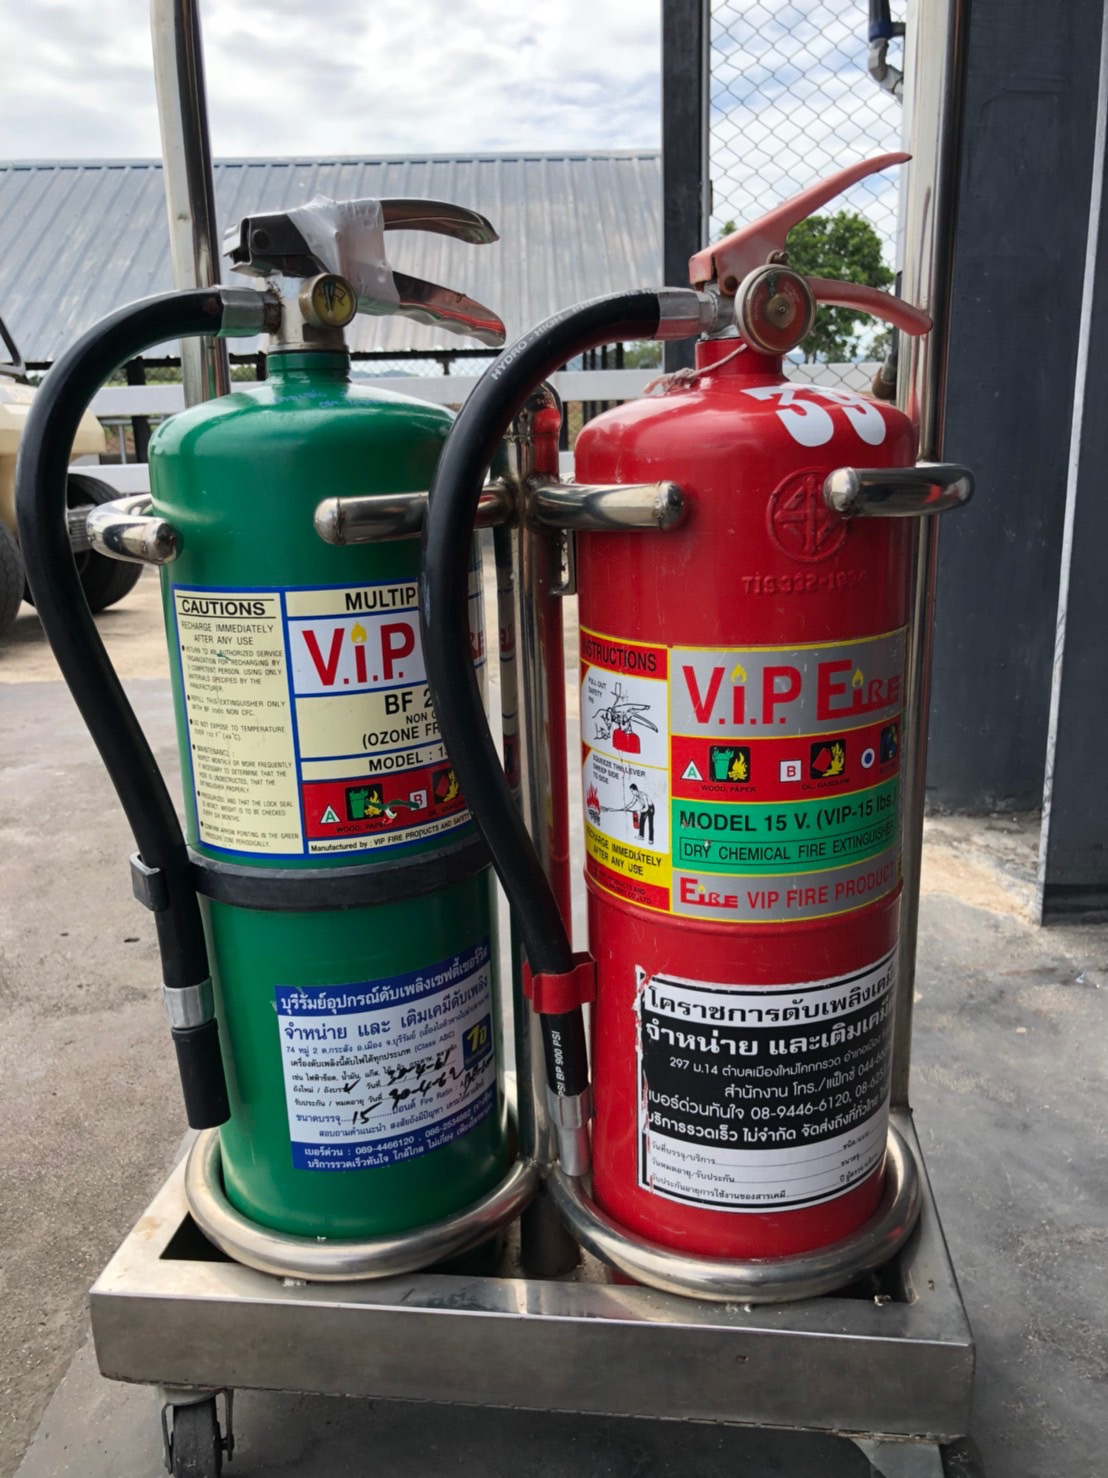
\includegraphics[width=0.4\linewidth]{images/Fire_Extinguisher.jpg}
\caption{ตัวอย่างถังดับเพลิงประจำสนามบินส่วนบุคคลขนงพระ}
\label{ตัวอย่างถังดับเพลิงประจำสนามบินส่วนบุคคลขนงพระ}
\end{center}
\end{figure}
	% Chapter 3: Aerodrome Data for AIS Report
%!TEX TS-program = xelatex
%!TEX encoding = UTF-8 Unicode

\chapter{ข้อมูลเกี่ยวกับแผนการจัดการสนามบินส่วนบุคคล}


\textbf{Programs and Procedures for Operating Private Aerodrome}

\section{แผนควบคุมตรวจสอบด้านความปลอดภัย (Aerodrome Safety Program)}

\subsection{การตรวจพินิจพื้นที่เคลื่อนไหว (Aerodrome Inspection)}

\subsubsection{รายละเอียดการดำเนินการตรวจพินิจต่างๆ} \label{รายละเอียดการดำเนินการตรวจพินิจต่างๆ}

วัตถุประสงค์การตรวจพินิจพื้นที่เคลื่อนไหว เพื่อให้เกิดความปลอดภัยแก่การบินขึ้น-ลงและเคลื่อนไหวของอากาศยาน การตรวจพินิจเป็นไปตามข้อกำหนดของสำนักงานการบินพลเรือนแห่งประเทศไทย การตรวจพินิจมีดังต่อไปนี้

\begin{enumerate}
\item การตรวจความสะอาดพื้นที่เคลื่อนไหว %
	\begin{enumerate}
		\item ตรวจพินิจพื้นที่เคลื่อนไหวทั่วไป (ทางวิ่ง ทางขับ ลานจอด) เป็นการตรวจสอบความสะอาดพื้นที่เคลื่อนไหวที่ปราศจากวัสดุแปลกปลอม (FOD) และสัตว์ที่อาจก่อให้เกิดความไม่ปลอดภัยต่อการขึ้น/ลง และการเคลื่อนไหวของอากาศยาน
		\item การตรวจพินิจพื้นที่เคลื่อนไหว มีความถี่ในการตรวจสอบ วันละ 1 ครั้ง ช่วงเช้า และ เมื่อมีความจำเป็น ก่อนอากาศยานทำการขึ้น – ลง การตรวจพินิจพื้นที่เคลื่อนไหว ใช้แบบรายงานการตรวจสอบ KNP-Form-01
	\end{enumerate}

\item การตรวจความฝืดบนทางวิ่ง %
	\begin{enumerate}
		\item การตรวจความฝืดบนทางวิ่ง มีวัตถุประสงค์เพื่อประเมินสภาพพื้นผิวทางวิ่ง ว่ามี friction เพียงพอที่จะไม่เกิดการลื่นไถลของอากาศยาน
		\item เนื่องจาก อากาศยานที่ขึ้นลง ณ สนามบินส่วนบุคคลขนงพระ เป็นอากาศยานขนาดเล็ก การ Touch down ไม่ทำให้มีรอยคราบยางที่จะลดความฝืดของทางวิ่ง
		\item แรงเสียดทานของผิวทางวิ่ง อาจจะลดลงเมื่อมีฝนตกและทางวิ่งเปียก  ซึงเป็นการตรวจในเรื่องปริมาณน้ำขังบนทางวิ่ง
	\end{enumerate}

\item การตรวจวัดปริมาณน้ำขังบนทางวิ่ง (Runway) และ ทางขับ (Taxiway) %
	\begin{enumerate}
		\item การการตรวจวัดปริมาณน้ำขังบนทางวิ่ง กระทำทุกครั้งหลังฝนตกหรือขณะฝนตก  ผู้รับผิดชอบการตรวจจะทำการตรวจสอบปริมาณน้ำขังบนทางวิ่งด้วยสายตาและจะแจ้งปริมาณน้ำขังบนทางวิ่งให้นักบินทราบทันที หากมีการทำการบินในช่วงเวลานั้น รวมถึงจะมีการใช้อุปกรณ์ไล่น้ำที่ขังออกจากพื้นผิวทางวิ่ง(ถ้ามี) เมื่อเห็นว่าปริมาณน้ำขังบนทางวิ่งนั้นอาจจะก่อให้เกิดอันตรายกับอากาศยานที่ทำการขึ้น-ลง 
		\item การแจ้งสภาพน้ำบนทางวิ่งและ ทางขับ (Taxiway) มี 4 ระดับ มีดังนี้
			\begin{description}
				\item[Damp:] ชื้น พื้นผิวเลี่ยนเป็นสีเข้มขึ้นเนื่องจากความชื้น
				\item[Wet:] เปียก พื้นผิวทางวิ่งเปียกแต่ไม่มีน้ำขัง
				\item[Water Patches:] มีน้ำขัง มองเห็นน้ำขังเป็นหย่อมๆ บนทางวิ่ง
				\item[Flooded:] น้ำท่วม มีน้ำขังบนทางวิ่ง
			\end{description}
	\end{enumerate}

\item การตรวจสภาพสนามหญ้าที่เป็น Runway strip และลานจอดอากาศยาน %
	ผู้รับผิดชอบจะตรวจสอบสภาพความเรียบร้อยของพื้นที่สนามหญ้า หรือที่ๆ ซึ่งมีหญ้าปกคลุมเป็นประจำทุกวัน พื้นที่บริเวณใดมีหญ้าปกคลุมจำนวนมากหรือหญ้าเจริญเติบโตมีส่วนสูงเกินมาตรฐานที่กำหนด จะดำเนินการตัดหญ้าให้อยู่ในเกณฑ์
\end{enumerate}

\subsubsection{การเก็บรักษาสมุดปูมการตรวจพินิจและสถานที่เก็บสมุดปูม}

สมุดปูมการตรวจพินิจเก็บรักษาไว้ที่สำนักงาน

\subsubsection{รายละเอียดของรอบและระยะเวลาการตรวจพินิจ}

\begin{enumerate}
\item การตรวจพินิจต่างๆ ตาม \ref{รายละเอียดการดำเนินการตรวจพินิจต่างๆ} ดำเนินการ วันละ 1 ครั้ง แต่ละครั้งใช้เวลา ประมาณ 1-15 นาที
\item รายงานการตรวจพินิจ ทำโดยการลงผลการตรวจในแบบฟอร์ม KNP-Form-01  ทุกวัน
\item ผู้ทำการตรวจเซ็นชื่อลงในแบบฟอร์มทุกครั้ง
\item ผู้ทำการตรวจเสนอผู้จัดการสนามบิน เพื่อทราบทุกเดือน
\end{enumerate}

\subsubsection{บัญชีรายการตรวจพินิจ}

รายการตรวจพินิจ ของสนามบินส่วนบุคคลขนงพระ มีดังนี้

\begin{enumerate}
\item ทางวิ่ง 10/28
\item ทางขับ และ Apron Taxiway 
\item ลานจอดอากาศยาน
\item พื้นที่หญ้า
\item ถุงลม
\item สีเครื่องหมายบนทางวิ่ง
\item รั้ว
\item สิ่งกีดขวางต่อการบิน
\item สัตว์ที่อาจเข้ามาในพื้นที่และเป็นอันตรายต่อการบิน
\item ถังดับเพลิง
\item บุคคลแปลกหน้า
\end{enumerate}

\subsubsection{การจัดทำรายงานผลการตรวจพินิจ และการติดตามผล}

ผู้รับผิดชอบตรวจพินิจรายงานการตรวจโดยการลงผลการตรวจในแบบฟอร์ม KNP-Form-01 หากพบสิ่งปกติ มีหน้าที่แก้ไขทันที   แล้วแจ้งผลการแก้ไขด้วยวาจา ก่อนลงผลการดำเนินการลงในแบบ KNP-Form-01 ช่องหมายเหตุ

หากไม่สามารถแก้ไขได้  ผู้รับผิดชอบตรวจพินิจจะรายงานผู้จัดการสนามบิน เพื่อทราบ และผู้จัดการสนามบิน เป็นผู้รับผิดชอบแก้ไข

เมื่อการแก้ไขเรียบร้อย ผู้รับผิดชอบตรวจพินิจผลการดำเนินการลงในแบบ KNP-Form-01 ช่องหมายเหตุ ระบุวันเวลาที่แก้ไขเสร็จเรียบร้อย

\subsubsection{ชื่อและตำแหน่งผู้มีหน้าที่รับผิดชอบการตรวจพินิจ }

ผู้มีหน้าที่รับผิดชอบทั้งในและนอกเวลาทำการ 
\begin{quote}
	\pgfornament[color=red!40!black, scale=0.25]{14} นายสุรชัย เงื้อมกลาง ผู้ดูแลสนามบิน หมายเลขโทรศัพท์ 097 965 9897
\end{quote}

\begin{landscape}
\subsection{แบบฟอร์ม KNP-Form-01 รายงานการตรวจพินิจพื้นที่เคลื่อนไหว}

\begin{table}[h!]
\caption{ตัวอย่าง KNP-Form-01 รายงานการตรวจพินิจพื้นที่เคลื่อนไหว}
\begin{center}
\begin{tabular}{|c|c|c|c|c|c|c|c|c|c|c|c|c|c|c|c|c|c|}
\hline
\multirow{3}{*}{วัน/เดือน/ปี} & \multirow{3}{*}{เวลาตรวจ}  & \multicolumn{2}{c|}{\multirow{3}{*}{สภาพทางวิ่ง}} &  \multicolumn{2}{c|}{\multirow{3}{*}{FOD}} &  \multicolumn{2}{c|}{ถุงลม} &  \multicolumn{2}{c|}{\multirow{3}{*}{สัตว์ในเขต}} &  \multicolumn{2}{c|}{\multirow{3}{*}{จุดน้ำขัง}} &  \multicolumn{2}{c|}{การบุกรุก} &  \multicolumn{2}{c|}{สิ่งปลูกสร้าง} & หมายเหตุ  & ลงชื่อ \\ % Heading row
 & & \multicolumn{2}{c|}{} & \multicolumn{2}{c|}{} & \multicolumn{2}{c|}{สีหมายเลขทางวิ่ง} & \multicolumn{2}{c|}{} & \multicolumn{2}{c|}{} & \multicolumn{2}{c|}{เขตพื้นที่} & \multicolumn{2}{c|}{อุปสรรค} & ระบุสิ่งไม่ปกติ & ผู้ตรวจพื้นที่ \\
 & & \multicolumn{2}{c|}{} & \multicolumn{2}{c|}{} & \multicolumn{2}{c|}{} & \multicolumn{2}{c|}{} & \multicolumn{2}{c|}{} & \multicolumn{2}{c|}{} & \multicolumn{2}{c|}{ต่อการบิน} & สิ่งที่พบและแก้ไข &  \\
\hline
 &  & ปกติ & ไม่ปกติ & มี & ไม่มี & ปกติ & ไม่ปกติ & พบ & ไม่พบ & มี & ไม่มี & มี & ไม่มี & มี & ไม่มี & & \\
 \hline
\textcolor{red}{ตัวอย่าง} & \textcolor{red}{ตัวอย่าง} & & & & & & & & & & & & & & & \textcolor{red}{ตัวอย่าง} &  \\
 \hline
\textcolor{red}{1/03/61} & \textcolor{red}{07:00 น.} & \textcolor{red}{\checkmark} & & & \textcolor{red}{\checkmark} & \textcolor{red}{\checkmark} & & & \textcolor{red}{\checkmark} & & \textcolor{red}{\checkmark} & & \textcolor{red}{\checkmark} & & \textcolor{red}{\checkmark} & & \\ \hline
\textcolor{red}{2/03/61} & \textcolor{red}{07:00 น.} & \textcolor{red}{\checkmark} & & \textcolor{red}{\checkmark} & & & & & & & \textcolor{red}{\checkmark} & & \textcolor{red}{\checkmark} & & \textcolor{red}{\checkmark} & \textcolor{red}{เศษหินบนทางวิ่ง} & \\
 & & & & & & & & & & & & & & & & \textcolor{red}{เก็บออกแล้ว} & \textcolor{red}{สุรชัย}\\ \hline
\textcolor{red}{2/03/61} & \textcolor{red}{16:30 น.} & \textcolor{red}{\checkmark} & & & & & & & & \textcolor{red}{\checkmark} & & & \textcolor{red}{\checkmark} & & \textcolor{red}{\checkmark} & \textcolor{red}{ฝนตกหนักไม่-} & \\ 
 & & & & & & & & & & & & & & & & \textcolor{red}{สามารถใช้สนามบิน} & \textcolor{red}{สุรชัย}\\ \hline
\end{tabular}
\end{center}
\label{KNP-Form-01 รายงานการตรวจพินิจพื้นที่เคลื่อนไหว}
\end{table}%
\textbf{การกรอก}
\begin{enumerate}
\item ระบุ วัน เวลา
\item ระบุ โดย check ปกติหรือไม่ปกติ    มีหรือไม่มี  พบหรือไม่พบ  หากไม่ปกติ     มีหรือพบ ให้ระบุในช่อง หมายเหตุ ว่า ไม่ปกติอย่างไร พบอะไร หรือ มีอะไร และ ได้แก้ไขไปอย่างไร
\item ลงชื่อ ทุกวัน  เมื่อครบเดือน ให้นำเสนอผู้ควบคุมสนามบิน
\item หากช่องกรอกไม่เพียงพอ ให้เขียนรายงานสิ่งที่ตรวจพบ และสิ่งที่ต้องแก้ไข แนบเพิ่มเติมได้ 
\end{enumerate}
ลงลายมือ ……………………………….......................... \\ 
ชื่อ-สกุล นายสุรชัย เงื้อมกลาง  %
\end{landscape}

\section{การตรวจพินิจเครื่องช่วยทัศนวิสัย (Aerodrome Visual Aids)}

สนามบินส่วนบุคคลขนงพระ ใช้งานเฉพาะในสภาพอากาศเปิด (VMC) 

สนามบินส่วนบุคคลขนงพระ  ไม่มี ระบบไฟฟ้าสนามบิน

การตรวจพินิจเครื่องช่วยทัศนวิสัย มีวัตถุประสงค์เพื่อให้ทราบสภาพของเครื่องช่วยทัศนวิสัย ให้อยู่ในสภาพที่ดี ใช้งานได้ เพื่อให้มีความปลอดภัย

\subsection{รายละเอียดการดำเนินการตรวจพินิจเครื่องช่วยทัศนวิสัย}\label{รายละเอียดการดำเนินการตรวจพินิจเครื่องช่วยทัศนวิสัย}

การตรวจพินิจเครื่องช่วยทัศนวิสัย  มีดำเนินรายละเอียดการดังนี้

\begin{enumerate}
\item เครื่องหมายบนทางวิ่ง \\
	ทำการตรวจ
	\begin{enumerate}
	\item ความชัดเจนของหมายเลขทางวิ่ง และเส้นกึ่งกลางทางวิ่ง
	\item สีของเครื่องหมายบนทางวิ่ง เป็นสีขาว
	\item ไม่มีสัญญลักษณ์แปลกปลอมอื่นบนทางวิ่ง เว้นแต่มีกรณีพิเศษ เช่น การปิดทางวิ่ง
	\end{enumerate}
\item เครื่องหมายบนทางขับ \\
	สนามบินขนงพระ เป็นสนามบินส่วนบุคคล ทางขับมีระยะทางสั้น จึงไม่จำเป็นต้องมี เครื่องหมายบนทางขับ อย่างไรก็ตาม การตรวจจะเป็นการตรวจว่าไม่มีสัญญลักษณ์แปลกปลอมอื่นบนทางขับ
\item ถุงลม \\
	สนามบินขนงพระ ใช้ ถุงลมสีส้ม จำนวน 2 ถุง ติดตั้งอยู่บริเวณกึ่งกลางทางวิ่งใกล้กับหอสังเกตการณ์ และหัวทางวิ่ง 10 บริเวณโรงเก็บอากาศยาน \\
	
ทำการตรวจโดยการสังเกต และใช้สายตาดู:
	\begin{enumerate}
	\item สีของถุงลม ยังคงมีสีส้มชัดเจน
	\item สภาพถุงลมอยู่ในสภาพดี 
	\item หมุนได้ตามทิศทางลม และยกตัวได้ตามความเร็วลม
	\end{enumerate}
\item ระบบไฟฟ้าสนามบิน \\
	ไม่มีระบบไฟฟ้าสนามบิน
\end{enumerate}

\subsection{การจัดการเพื่อดำเนินการตรวจพินิจเครื่องช่วยทัศนวิสัยรายการตรวจระหว่างทำการและนอกเวลาทำการปกติ และบัญชีรายการตรวจพินิจ}

\subsection{การจัดการ}

การตรวจพินิจเครื่องช่วยทัศนวิสัย  ระหว่างเวลาทำการ มีความถี่ในการตรวจสอบ วันละ 1 ครั้ง ช่วงเช้า และ เมื่อมีความจำเป็น ก่อนอากาศยานทำการขึ้น – ลง

\begin{enumerate}
\item การตรวจพินิจต่างๆ ตาม \ref{รายละเอียดการดำเนินการตรวจพินิจเครื่องช่วยทัศนวิสัย} ดำเนินการ วันละ 1 ครั้ง แต่ละครั้งใช้เวลา ประมาณ 10-15 นาที
\item รายงานการตรวจพินิจ ทำโดยการลงผลการตรวจในแบบฟอร์ม KNP-Form-01  ทุกวัน ช่องถุงลม/สีหมายเลขทางวิ่ง
\item ผู้ทำการตรวจเซ็นชื่อลงในแบบฟอร์มทุกครั้ง
\item ผู้ทำการตรวจเสนอผู้จัดการสนามบิน เพื่อทราบทุกเดือน
\end{enumerate}

โดยปกติ จะไม่มีการตรวจพินิจเครื่องช่วยทัศนวิสัยนอกเวลาทำการ แต่จะกระทำเมื่อมีกรณีพิเศษ เมื่อมีเหตุจำเป็น และการตรวจจะใช้วิธีการเช่นเดียวกับการตรวจตรวจในเวลาทำการ

\subsubsection{บัญชีรายการตรวจพินิจ}

สนามบินขนงพระ มีเครื่องช่วยทัศนวิสัย  อันได้แก่

\begin{enumerate}
\item เครื่องหมายบนทางวิ่ง
\item ถุงลม
\end{enumerate}

\subsection{การจัดทำรายงานผลตรวจพินิจและการติดตามผลเพื่อการแก้ไข}

ผู้รับผิดชอบตรวจพินิจรายงานการตรวจโดยการลงผลการตรวจในแบบฟอร์ม KNP-Form-01 ช่องถุงลม/สีหมายเลขทางวิ่ง    หากพบสิ่งปกติ มีหน้าที่แก้ไขทันที   แล้วแจ้งผลการแก้ไขด้วยวาจา ก่อนลงผลการดำเนินการลงในแบบ KNP-Form-01 ช่องหมายเหตุ

หากไม่สามารถแก้ไขได้  ผู้รับผิดชอบตรวจพินิจจะรายงานผู้จัดการสนามบิน เพื่อทราบ และผู้จัดการ เป็นผู้รับผิดชอบแก้ไข

เมื่อการแก้ไขเรียบร้อย ผู้รับผิดชอบตรวจพินิจผลการดำเนินการลงในแบบ KNP-Form-01 ช่องหมายเหตุ ระบุวันเวลาที่แก้ไขเสร็จเรียบร้อย

\subsection{การจัดการเพื่อดำเนินการบำรุงรักษาประจำและการบำรุงรักษาฉุกเฉิน}

การบำรุงรักษาเครื่องช่วยทัศนวิสัย ของสนามบินขนงพระ แบบประจำ มีการดำเนินการ ดังนี้

\begin{enumerate}
\item กวาดทางวิ่ง เป็นประจำ เพื่อให้มองเห็น เครื่องหมายบนทางวิ่ง ชัดเจน
\item เปลียนถุงลม เมื่อสีซีดจาง
\item หยอดสารหล่อลื่นจุดหมุนต่างของเสาถุงลมทุก 1 เดือน
\end{enumerate}

แบบเมื่อฉุกเฉิน มีการดำเนินการ ดังนี้

\begin{enumerate}
\item ทาสีเครื่องหมายบนทางวิ่งทันที หากมีเหตุที่ทำให้เครื่องหมายหายไป
\item เปลียนถุงลมทันที หากมีเหตุที่ทำให้ถุงลมใช้งานไม่ได้
\end{enumerate}

\subsection{การจัดการเกี่ยวกับเครื่องกำเนิดไฟฟ้าสำรอง และรายละเอียดของวิธีการอื่นๆที่ใช้จัดการในกรณีที่ระบบไฟฟ้าขัดข้องทั้งหมดหรือบางส่วน}

สนามบินขนงพระ เปิดใช้งานระหว่าง พระอาทิตย์ขึ้น ถึง พระอาทิตย์ตก ภายใต้สภาพอากาศเปิด (VMC) สนามบินขนงพระ ไม่มีไฟฟ้าสนามบิน จึงไม่ต้องมีเครื่องกำเนิดไฟฟ้าสำรอง

\subsection{ชื่อและตำแหน่งผู้มีหน้าที่รับผิดชอบการตรวจพินิจและดำเนินการบำรุงรักษาไฟฟ้า และหมายเลขโทรศัพท์ของผู้มีหน้าที่รับผิดชอบระหว่างเวลาทำการและนอกเวลาทำการของสนามบิน}

\subsubsection{ระหว่างเวลาทำการ (During Office Hours)}

นายสุรชัย เงื้อมกลาง ผู้ดูแลสนามบิน  หมายเลขโทรศัพท์ 097 965 9897

\subsubsection{นอกเวลาทำการ (Outside office hours)}

นายอติพล โหตระกิตย์ ผู้ช่วยผู้จัดการสนามบิน	หมายเลขโทรศัพท์ 089 478 0808

\section{การบำรุงรักษาพื้นที่เคลื่อนไหว (Movement Area Maintenance)}

พื้นที่เคลื่อนไหว (Movement area) หมายถึง ส่วนของสนามบินซึ่งใช้สำหรับการขึ้น/ลง และขับเคลื่อนของอากาศยาน ประกอบด้วยทางวิ่ง ทางขับ และลานจอดอากาศยาน

วัตถุประสงค์ของการบำรุงรักษาพื้นที่เคลื่อนไหวของสนามบินขนงพระ คือเพื่อรักษาสภาพพื้นที่ให้อยู่ในสภาพใช้งานได้ตลอดเวลาอย่างปลอดภัย และเป็นไปตามสำนักงานการบินพลเรือนแห่งประเทศไทยกำหนด

\subsection{รายละเอียดของสิ่งอำนวยความสะดวกและวิธีการดำเนินงานเพื่อบำรุงรักษาพื้นที่เคลื่อนไหว}

สิ่งอำนวยความสะดวกของสนามบินขนงพระ มีรายละเอียด ดังนี้

\begin{enumerate}
\item พื้นที่ที่ต้องทำการบำรุงรักษา
	\begin{enumerate}
	\item พื้นที่มีผิวจราจร (Paved area) ได้แก่ ทางวิ่ง 10/28 ทางขับ
	\item พื้นที่ที่ไม่มีผิวจราจร (Unpaved Area) ได้แก่ ลานจอดอากาศยาน พื้นที่ปลอดภัยรอบทางวิ่งและรอบทางขับ
	\item รั้วเขตการบิน
	\end{enumerate}
\item อุปกรณ์ทำการบำรุงรักษา
	\begin{enumerate}
	\item รถตัดหญ้า
	\item รถแทรคเตอร์ขนาดเล็ก
	\item ไม้กวาด
	\end{enumerate}
\end{enumerate}

วิธีการบำรุงรักษาพื้นที่เคลื่อนไหว เป็นไปตาม หัวข้อ \ref{การบำรุงรักษาพื้นที่ที่มีผิวทาง (Paved Area)}, \ref{การบำรุงรักษาพื้นที่ที่ไม่มีผิวทาง (Unpaved Area)},  \ref{การบำรุงรักษาพื้นที่ปลอดภัยรอบทางวิ่ง (Runway Strip) และปลอดภัยรอบทางขับ (Taxiway Strip)} และ \ref{การบำรุงรักษาระบบระบายน้ำของสนามบิน}

\subsection{การบำรุงรักษาพื้นที่ที่มีผิวทาง (Paved Area)} \label{การบำรุงรักษาพื้นที่ที่มีผิวทาง (Paved Area)}

การบำรุงรักษาพื้นที่มีผิวจราจร (Paved area) มีดังนี้

\begin{enumerate}
\item ผู้รับผิดชอบตามหัวข้อ \ref{ชื่อและตำแหน่งผู้มีหน้าที่รับผิดชอบการบำรุงรักษาพื้นที่เคลื่อนไหว และหมายเลขโทรศัพท์ของผู้มีหน้าที่รับผิดชอบระหว่างเวลาทำการและนอกเวลาทำการของสนามบิน} ทำการตรวจสอบสภาพสนามบิน ทุกวัน โดยการตรวจสอบด้วยสายตา ทุกวัน ก่อนอากาศยานทำการบิน ขึ้น– ลง
\item การทำความสะอาดลานจอดอากาศยาน โดยใช้ไม้กวาดและเก็บ FOD ในระหว่างวันทำการและนอกเวลาทำการ ดูแลความสะอาดในลานจอดและทางวิ่ง ทางขับ หรือออกปฏิบัติงานเพิ่มเติมได้เมื่อเห็นสมควร หรือมีผู้ร้องขอ
\item เมื่อพบการชำรุดของผิวจราจรจะดำเนินการปิดซ่อมแซมพื้นที่ด้วยวัสดุแอสฟัส Cold Mix หรือ Hot Mix สำเร็จรูป หรือวัสดุที่เหมาะสมตามหลักวิศวกรรม
\item เมื่อตรวจพบว่าสภาพโครงสร้างพื้นฐานของผิวจราจรเสียหาย จะทำการซ่อมแซมใหญ่โดยจ้างช่างภายนอก การดำเนินการดังกล่าวจะประสานผู้มาทำการบินเพื่อแจ้งให้ทราบล่วงหน้าตามระยะเวลาที่คาดการเบื้องต้น
\end{enumerate}

\subsection{การบำรุงรักษาพื้นที่ที่ไม่มีผิวทาง (Unpaved Area)}\label{การบำรุงรักษาพื้นที่ที่ไม่มีผิวทาง (Unpaved Area)}

การบำรุงรักษาพื้นที่ไม่มีผิวจราจร (Unpaved Area) มีดังนี้

\begin{enumerate}
\item ตรวจสอบและปรับพื้นที่ไหล่ทางวิ่ง ทางขับ และลานจอด ให้ได้ความลาดเอียงเพื่อการระบายน้ำออกนอกพื้นที่ รวมทั้งกลบหลุมบ่อเพื่อความปลอดภัยของอากาศยานเมื่อเกิดอุบัติเหตุวิ่งออกนอกทางวิ่ง ทางขับ
\item ตัดหญ้าพื้นที่เขต AIRSIDE โดยพนักงานของสนามบินขนงพระ ซึ่งควบคุมความสูงของหญ้าไม่ให้เกิน ๕-๑๐ ซม. 
\item กำจัดและควบคุมพื้นที่ที่ไม่มีพื้นผิวทางจราจร (Unpaved Area) ซึ่งเป็นแหล่งอาหารของนกและสัตว์อื่นๆ เพื่อป้องกันการเพิ่มของนกและควบคุมมิให้สัตว์ เข้ามาในเขตการบิน เช่น สร้างรั้วโดยรอบ
\item ควบคุมความสูงของพุ่มไม้และต้นไม้ ให้อยู่ในเกณฑ์ความปลอดภัยการทำการบิน
\end{enumerate}

\subsection{การบำรุงรักษาพื้นที่ปลอดภัยรอบทางวิ่ง (Runway Strip) และปลอดภัยรอบทางขับ (Taxiway Strip)}\label{การบำรุงรักษาพื้นที่ปลอดภัยรอบทางวิ่ง (Runway Strip) และปลอดภัยรอบทางขับ (Taxiway Strip)}

การบำรุงรักษาพื้นที่ปลอดภัยรอบทางวิ่ง และรอบทางขับ มีดังนี้

\begin{enumerate}
\item ตัดหญ้าให้สั้น ทุก ๓๐ วัน บริเวณเขตทางวิ่ง ทางขับ เก็บหญ้าที่ตัดออก เพื่อป้องกันปลิวเข้าทางวิ่ง ทางขับ
\item รถแทรกเตอร์ที่ใช้ในการตัดหญ้า รวมทั้งรถอื่นๆ ที่ร่วมเข้าตัดหญ้า ให้ติดธงตราหมากรุก และเข้าทำงานในช่วงเวลาไม่มีการทำการบิน 
\end{enumerate}

\subsection{การบำรุงรักษาระบบระบายน้ำของสนามบิน}\label{การบำรุงรักษาระบบระบายน้ำของสนามบิน}

การบำรุงรักษาระบบระบายน้ำ เพื่อให้มีระบายน้ำผิวดินออกจากพื้นที่เคลื่อนไหว มีการดำเนินงาน โดย ให้พนักงานสำรวจเส้นทางระบายน้ำในเขตการบิน แบ่งเป็นช่วง ก่อนฤดูฝน ระหว่างฤดูฝน และหลังฤดูฝน สำรวจเส้นทางระบายน้ำนอกเขตการบินช่วงเวลาก่อนฤดูฝน  หากตรวจพบวัชพืช ความตื้นเขินหรือสิ่งอื่นใดที่ขัดขวางการไหลของน้ำต้องกำจัดทันที

\subsection{ชื่อและตำแหน่งผู้มีหน้าที่รับผิดชอบการบำรุงรักษาพื้นที่เคลื่อนไหว และหมายเลขโทรศัพท์ของผู้มีหน้าที่รับผิดชอบระหว่างเวลาทำการและนอกเวลาทำการของสนามบิน} \label{ชื่อและตำแหน่งผู้มีหน้าที่รับผิดชอบการบำรุงรักษาพื้นที่เคลื่อนไหว และหมายเลขโทรศัพท์ของผู้มีหน้าที่รับผิดชอบระหว่างเวลาทำการและนอกเวลาทำการของสนามบิน}

\subsubsection{ระหว่างเวลาทำการ Office Hours}

นายนิวัฒน์ ถี่ถ้วน Supervisor งานโยธา 	หมายเลขโทรศัพท์ 064 682 2838

\subsubsection{นอกเวลาทำการ Outside office hours}

นายอติพล โหตระกิตย์ ผู้ช่วยผู้จัดการสนามบิน	หมายเลขโทรศัพท์ 089 478 0808

\section{การควบคุมสิ่งกีดขวาง (Obstacle Control)}

การควบคุมสิ่งกีดขวาง เพื่อมิให้สิ่งกีดขวางที่อาจก่อให้เกิดความไม่ปลอดภัยต่อการขึ้น-ลง และการเคลื่อนไหวของอากาศ-ยาน ได้แก่ อาคาร เสาไฟฟ้า สิ่งปลูกสร้าง ต้นไม้ยืนต้น ฯลฯ

\subsection{รายละเอียดวิธีดำเนินการควบคุมสิ่งกีดขวาง}

สนามบินขนงพระ เป็นสนามบินส่วนบุคคล ไม่ได้รับการประกาศให้บริเวณใกล้เคียงสนามบินเป็นเขตปลอดภัยในการเดินอากาศ

ที่ดินโดยรอบสนามบินขนงพระเป็นสนามกอล์ฟ Rancho Charnvee Resort and Country Club (รูปที่ \ref{แผนผังแนวเขตสนามบินขนงพระ อำเภอปากช่อง จังหวัดนครราชสีมา}) จึงไม่มีการก่อสร้างอาคารหรือสิ่งกีดขวางที่มีความสูง โดยบริเวณปลายทางวิ่ง 10 และทางวิ่ง 28 พื้นดินโดยรอบมีค่าระดับต่ำกว่าระดับ Threshold ของทางวิ่ง ทำให้การก่อสร้างอาคารสิ่งปลูกสร้างตามปกติจะไม่มีผลกับการปฏิบัติการบินที่สนามบินขนงพระ

\subsection{การเฝ้าระวังสิ่งกีดขวางในระนาบจำกัดสิ่งกีดขวาง และในระนาบการวิ่งขึ้นของ
อากาศยาน}\label{การเฝ้าระวังสิ่งกีดขวางในระนาบจำกัดสิ่งกีดขวาง และในระนาบการวิ่งขึ้นของ
อากาศยาน}

\begin{enumerate}
\item ระนาบจำกัดสิ่งกีดขวาง ของสนามบินขนงพระ มีรายละเอียดดั่งปรากฏในตารางที่ \ref{ระนาบจํากัดสิ่งกีดขวาง ของสนามบินขนงพระ}

\begin{table}[h!]
\caption{ระนาบจํากัดสิ่งกีดขวาง ของสนามบินขนงพระ}
\begin{center}
\begin{tabular}{lll}
& & \\
Conical surface	& & \\
 & Slope & 5\% \\
 & Height & 35m. \\
Inner Surface & & \\
 & Height & 45m. \\
 & Radius & 2,000 m. \\
Approach Surface & & \\
 & Length of inner edge & 60m. \\
 & Distance of threshold & 30m. \\
 & Divergence (each side)	& 10\% \\
 & First section length & 1,600m. \\
 & First section slope	 & 5\% \\
Take-off Surface & & \\
 & Length of inner edge & 60 m. \\	
 & Distance of threshold & 30m. \\
 & Divergence (each side) & 10\% \\
 & First section length & 1,600m. \\
 & First section slope	 & 5\% \\
 & Final width & 380m. \\
\end{tabular}
\end{center}
\label{ระนาบจํากัดสิ่งกีดขวาง ของสนามบินขนงพระ}
\end{table}%

\item บริเวณ Inner Horizontal surface มีกลุ่มต้นไม้ ตามภาพแสดงในแปลนสนามบิน ในหัวข้อ \ref{แผนผังสนามบินแสดงแนวเขตสนามบิน} แต่เนื่องจากการทำการบินที่สนามบินขนงพระเป็นการบินด้วยอากาศยานส่วนบุคคล ในลักษณะการบินแบบ VFR   การทำการบินจึงสามารถควบคุมให้อยู่ในเกณฑ์ปลอดภัย
\item การเฝ้าระวัง ทำโดยการตรวจสำรวจสิ่งกีดขวางภายในพื้นผิวเขตจำกัดสิ่งกีดขวางของสนามบินขนงพระ โดยเฉพาะแนวร่อน (Approach Surface)  และแนววิ่งขึ้น (Take-off Climb Surface) ของแต่ละทางวิ่ง โดยการสังเกตทุกวัน
\end{enumerate}

\subsection{การควบคุมสิ่งกีดขวางตามอำนาจหน้าที่ของเจ้าของหรือผู้ดำเนินงานสนามบิน}

ที่ดินโดยรอบสนามบินขนงพระ เป็นสนามกอล์ฟ Rancho Charnvee Resort and Country Club จึงไม่มีผลกระทบต่อการทำการบินด้วยอากาศยานส่วนบุคคล ในลักษณะการบินแบบ VFR   

นอกจากนี้ พื้นที่บริเวณห่างไกลออกไป มีสภาพเป็นไร่สวนปลูกไม้ล้มลุก จึงไม่มีผลกระทบต่อการปฏิบัติการบินเช่นกัน
หน่วยงานที่มีอำนาจควบคุมการปลูกสร้างในท้องที่อำเภอขนงพระ คือ องค์การบริหารส่วนตำบลขนงพระ 

\subsection{การเฝ้าระวังความสูงของอาคารหรือสิ่งก่อสร้างในพื้นที่โดยรอบระนาบจำกัดสิ่งกีดขวาง}

ดำเนินการเช่นเดียวกับ หัวข้อ \ref{การเฝ้าระวังสิ่งกีดขวางในระนาบจำกัดสิ่งกีดขวาง และในระนาบการวิ่งขึ้นของ
อากาศยาน}

\subsection{การแจ้งสำนักงานเกี่ยวกับสภาพและที่ตั้งของสิ่งกีดขวาง และการเคลื่อนย้ายหรือการต่อเติมใดๆ ที่เกิดขึ้นภายหลังที่เห็นว่าจำเป็น}

กรณีที่มีสิ่งกีดขวางที่อาจเป็นอุปสรรคต่อการบิน สนามบินขนงพระ จะแจ้งสำนักงานการบินพลเรือนแห่งประเทศไทย โดยทันที ไปยังหมายเลขโทรศัพท์ 02 568 8800 

\section{แผนการบริหารจัดการอันตรายที่เกิดจากสัตว์ (Wildlife Hazard Management Program)}

\subsection{การจัดการเพื่อประเมินอันตรายจากสัตว์}

จากการที่สนามบินขนงพระ ได้รับการอนุญาตเป้นที่ขึ้นลงชั่วคราวของอากาศยานอย่างต่อเนื่องมามากกว่า 4 ปี ทางสนามบินได้มีการสังเกตและประเมินพบว่า สัตว์ที่อาจเป็นอันตรายต่อการทำการบินได้แก่

\begin{enumerate}
\item นก
\item สุนัข (เป็นสัตว์เลี้ยง)
\end{enumerate}

\subsection{การจัดการเพื่อปฏิบัติให้เป็นไปตามแผนงานควบคุมสัตว์}

การจัดการควบคุมสัตว์ที่เป็นอันตรายต่อการทำการบิน มีดังนี้

\begin{enumerate}
\item การจัดการด้านสิ่งแวดล้อม \\
การจัดการด้านสิ่งแวดล้อมเพื่อป้องกันไม่ให้มีสิ่งดึงดูดนก และสัตว์ ได้แก่ การตัดหญ้า การเลือกชนิดต้นไม้เพื่อปลูก การทำความสะอาด การจัดเก็บขยะ
\item การควบคุมขับไล่ \\
ทำการตรวจสอบและติดตามการเพิ่มจำนวนของนกและสัตว์ การเปลี่ยนแปลงของสภาพแวดล้อมภายในสนามบิน ดำเนินการจับหรือขับไล่ด้วยวิธีต่างๆ เช่น ใช้ประทัดและแตร ทำให้เกิดเสียงดังขับไล่ ตรวจอาคารอยู่เสมอเพื่อป้องกันไม่ให้เป็นที่เกาะพักของนก
\item การแจ้งเตือนอันตรายจากนก \\
เมื่อพบว่าจะเป็นอันตรายต่อการทำการบิน จะแจ้งให้นักบินทราบทางวิทยุสื่อสาร
\item การดำเนินการเมื่ออากาศยานชนนกในพื้นที่
	\begin{enumerate}
	\item เข้าตรวจสอบบริเวณพื้นที่ที่ได้รับรายงานและดำเนินการเก็บซากและเข้าตรวจสอบอากาศยานที่ชนนกร่วมกับช่างว่าได้รับความเสียหายหรือไม่ พร้อมทั้งบันทึกภาพร่องรอยการชน
	\item แจ้งนักบินให้รายงานการเกิดอุบัติเหตุอากาศยานชนนกให้สำนักงานการบินพลเรือนแห่งประเทศไทยทราบโดยเร็ว ตามแบบ Bird Strike Reporting Form ของสำนักงานการบินพลเรือนแห่งประเทศไทย (รูปที่ \ref{Bird Strike Reporting Form} หน้าที่ \pageref{แบบฟอร์ม Bird Strike Report Form ของ สำนักงานการบินพลเรือนแห่งประเทศไทย})
	\end{enumerate}
\item มาตรการป้องกันอันตรายจากสัตว์
สนามบินขนงพระ มีรั้วและแนวคันดินที่ใช้ป้องกันสัตว์เข้ามาในเขตสนามบิน โดยเจ้าหน้าที่ประจำหอสังเกตการณ์จะตรวจสอบสัตว์ในบริเวลณทางวิ่งตลอดเวลา
\end{enumerate}

\subsection{ชื่อและตำแหน่งของผู้ที่มีหน้าที่รับผิดชอบเกี่ยวกับอันตรายที่เกิดจากสัตว์
และหมายเลขโทรศัพท์ของบุคคลที่มีหน้าที่รับผิดชอบในระหว่างเวลาทำการและนอกเวลาทำการของสนามบิน}

\subsubsection{ระหว่างเวลาทำการ (During Office Hours)}

นายสุรชัย เงื้อมกลาง ผู้ดูแลสนามบิน หมายเลขโทรศัพท์ 097 965 9897


\subsubsection{นอกเวลาทำการ (Outside office hours)}

นายอติพล โหตระกิตย์ ผู้ช่วยผู้จัดการสนามบิน	หมายเลขโทรศัพท์ 089 478 0808

\section{แผนการรักษาความปลอดภัยสนามบินส่วนบุคคล (Aerodrome Security Program)}

\subsection{วัตถุประสงค์ของแผนรักษาความปลอดภัย}

แผนรักษาความปลอดภัยสนามบินส่วนบุคคลขนงพระ มีวัตถุประสงค์ 

\begin{enumerate}
\item เพื่อป้องกันการกระทำโดยไม่ชอบด้วยกฎหมาย ในเขตสนามบินขนงพระ หรือ ใช้สนามบินขนงพระเพื่อนำไปสู่การกระทำโดยไม่ชอบด้วยกฎหมายที่จะเป็นอันตรายต่อการบินพลเรือน
\item เพื่อเพิ่มความปลอดภัยในการดำเนินงานของสนามบินตามข้อกำหนดของกฎกระทรวงว่าด้วยการขอและออกใบอนุญาตจัดตั้งสนามบิน พ.ศ 2560 และเพื่อให้ป็นไปตามประกาศสำนักงานการบินพลเรือนแห่งประเทศไทย เรื่อง มาตรฐานคู่มือสนามบินส่วนบุคคล พ.ศ. 2561
\end{enumerate}

สนามบินขนงพระ เป็นสถานที่ส่วนบุคคล การเข้าพื้นที่ต้องได้รับอนุญาต 

ผู้จัดการสนามบินและผู้ที่ได้รับมอบหมายจากผู้จัดการสนามบินให้ปฏิบัติหน้าที่ด้านการรักษาความปลอดภัยที่สนามบิน  เป็น ผู้รับผิดชอบด้านการรักษาความปลอดภัยสนามบิน

ผู้ที่ไม่ได้เกี่ยวข้องกับการรักษาความปลอดภัยโดยตรง (Non-Security Personnel) จะอยู่ในพื้นที่สนามบินได้ คือ ผู้ที่ทำงานภายในสนามบิน หรือ ผู้ที่ได้รับอนุญาตเข้าใช้สนามบิน มีหน้าที่ และความรับผิดชอบ ที่ต้องแจ้งผู้จัดการสนามบิน เมื่อพบเห็นการรุกล้ำของบุคคลแปลกหน้า หรือ บุคคลที่ไม่ได้รับอนุญาตอยู่ในเขตสนามบิน

เมื่อมีเหตุการเกิดขึ้นทางด้านการรักาความปลอดภัย ผู้ที่ไม่ได้เกี่ยวข้องกับการรักษาความปลอดภัยโดยตรง (Non-Security Personnel) จะต้องปฏิบัติตาม วิธีการเผชิญเหตุ ที่ผู้จัดการฯ นำมาปฏิบัติใช้

\subsection{การคัดกรองบุคลากรและการฝึกอบรมของบุคลากร}

การรับบุคคลเข้าทำงานในสนามบิน จะต้องเป็นผู้ที่ผ่ารการตรวจสอบประวัติอาชญากรรมและประวัติการทำงานย้อนหลัง เช่นเดียวกับการรับพนักงานของบริษัทต่างๆ

สนามบินขนงพระเป็นสถานที่ส่วนบุคคล  และก่อนการปฏิบัติงานผู้ที่ได้รับมอบหมายให้ปฏิบัติงานที่สนามบินจะต้องได้รับการอบรม (Briefing) จากผู้จัดการสนามบิน ให้ทราบถึงขอบเขต กระบวนการเข้าออกสนามบิน โรงเก็บอากาศยาน และพื้นที่ต่างๆของสนามบิน รวมทั้งการแจ้งเหตุต่อผู้จัดการ ไปยังสถานีตำรวจ และสำนักงานการบินพลเรือนแห่งประเทศไทย

\subsection{การเข้าพื้นที่เคลื่อนไหวของสนามบิน (Access to Aerodrome Movement Area)}

\subsubsection{\underline{\textcolor{red}{เขตพื้นที่หวงห้าม}}}

สนามบินขนงพระเป็นสถานที่ส่วนบุคคล  พื้นที่สนามบินทั้งหมดมีการแสดงเขตแนวด้วยรั้ว ไม้กั้น และคันดิน 

แนวรั้ว ไม้กั้น และคันดิน สามารถแสดงให้บุคคลที่ไม่เกี่ยวข้องรับทราบเขตปฏิบัติการบิน โดยมีการแสดงป้ายระบุเขตพื้นที่ปฏิบัติการบินตามจุดโดยรอบ ซึ่งสามารถป้องกันทั้งคนและสัตว์ที่จะเข้าถึงเขตหวงห้าม นอกจากนี้รอบนอกเขตสนามบินโดยส่วนใหญ่ก็ยังเป็นที่ดินของสนามกอล์ฟ Rancho Charnvee Resort and Country Club ซึ่งมีระบบรักษาความปลอดภัยเข้มงวดและมีพนักงานปฏิบัติงานเป็นจำนวนมาก นับได้ว่ามีการป้องกันการเข้าถึงพื้นที่สนามบินถึง 2 ชั้น 

\subsubsection{\underline{\textcolor{red}{ควบคุมการเข้า - ออก}}}

การเข้า – ออกสนามบินสามารถทำได้ 2 ช่องทาง โดย

\begin{enumerate}
\item การเข้าออกผ่านทางสนามกอล์ฟ Rancho Charnvee Resort and Country Club สำหรับผู้เกี่ยวข้อง ซึ่งมีระบบรักษาความปลอดภัยโดยเจ้าหน้าที่ รปภ. ระบบไม้กั้น และป้ายแจ้งห้ามผู้ไม่เกี่ยวข้องผ่าน 
\item การผ่านพื้นที่สนามบินโดยทางสาธารณะ ซึ่งจะมีเจ้าหน้าที่ไปประจำบริเวณทางผ่านเมื่อมีกิจกรรมการบิน และมีป้ายระบุเขตการบิน
\end{enumerate}

ยานพาหนะ ต้องจอดในที่ที่กำหนดเท่านั้น    ผู้โดยสารหรือผู้จะทำการบินมีที่พักคอย ณ ที่สำนักงานสนามบิน
สนามบินได้จัดทำป้ายแสดงเขตพื้นที่หวงห้าม ตามพื้นที่ที่กำหนดให้เห็นชัดเจน

\subsubsection{\underline{\textcolor{red}{บุคลากรผู้รับผิดชอบในการปฏิบัติหน้าที่รักษาความปลอดภัย}}}

\textbf{ระหว่างเวลาทำการ (During Office Hours)}

นายสุรชัย เงื้อมกลาง ผู้ดูแลสนามบิน หมายเลขโทรศัพท์ 097 965 9897

\textbf{นอกเวลาทำการ (Outside office hours)}

นายอติพล โหตระกิตย์ ผู้ช่วยผู้จัดการสนามบิน หมายเลขโทรศัพท์ 089 478 0808

ผู้ประจำหน้าที่หรือผู้ปฏิบัติงานในอากาศยานจะต้องไม่มีวัตถุผิดกฎหมาย หรือวัตถุต้องห้ามด้านการบินพลเรือน  

ผู้ประจำหน้าที่หรือผู้ปฏิบัติงานในอากาศยาน ผู้โดยสาร สัมภาระ หรือสิ่งของที่จะไปกับอากาศยาน ต้องแสดงตนและประกาศตนว่าไม่มีวัตถุผิดกฎหมาย หรือวัตถุต้องห้ามด้านการบินพลเรือน หากจำเป็น จะต้องถูกตรวจค้นด้วยมือ  นอกจากนี้ หากมีการนำอากาศยานไปลงจอด ณ สนามบินพาณิชย์ นักบินและผู้โดยสาร พร้อมสัมภาระ ต้องจอดแยกจากอากาศยานพาณิชย์ และปฏิบัติตามมาตรการรักษาความปลอดภัยของสนามบินพาณิชย์แห่งนั้นๆ

\subsubsection{\underline{\textcolor{red}{แผนเผชิญเหตุ (Contingency Plan)}}}

กรณีพบเหตุหรือสิ่งของต้องสงสัย
หากพบเหตุการณ์ สิ่งของ หรือพฤติกรรมที่น่าสงสัยที่สนามบิน จะแจ้งสถานีตำรวจภูธรหนองสาหร่าย ต.หนองสาหร่าย อ.ปากช่อง จ.นครราชสีมา หมายเลขโทรศัพท์ 044 938 794 โดยทันที

หากสนามบินได้รับแจ้งการขู่วางระเบิดหรือภัยคุกคามอื่นๆที่อาจก่อให้เกิดการกระทำอันเป็นการแทรกแซงโดยมิชอบด้วยกฎหมาย สนามบินจะประเมินสถานการณ์ภัยคุกคามดังกล่าวและแจ้งสถานีตำรวจภูธรหนองสาหร่าย ต.หนองสาหร่าย อ.ปากช่อง จ.นครราชสีมา หมายเลขโทรศัพท์ 044 938 794 โดยทันที

\subsubsection{\underline{\textcolor{red}{การประเมินความเสี่ยง (Risk Assessment)  ของภัยคุกคามที่อาจเกิดขึ้น}}}

สนามบินขนงพระ มีภัยคุกคามในระดับต่ำ ประเมินจากสภาพแวดล้อม ประสบการณ์การดำเนินการสนามบินที่ผ่านมา หน่วยงานท้องถิน และสถานีตำรวจ ดังนี้

\begin{table}[ht]
\caption{การประเมิความเสี่ยงสนามบินขนงพระ}
\begin{center}
\begin{tabular}{ll}
& \\
สภาพแวดล้อม & : เป็นสนามกอล์ฟ ไร่นา ทุ่งนา	\\
การดำเนินการสนามบินที่ผ่านมา & : ไม่มีภัยคุกคาม \\
หน่วยงานท้องถิน และสถานีตำรวจ & : ไม่มีการกระทำผิดกฏหมายในเขตสนามบิน \\
ทรัพย์สิน/อากาศยาน & : แรงจูงใจให้ทำผิดกฏหมายไม่มี \\
				& -เนื่องจากนำออกนอกสนามบินไม่ได้ \\
การป้องกันของสนามบิน & : อยู่ในระดับสูง \\
\end{tabular}
\end{center}
\label{การประเมิความเสี่ยงสนามบินขนงพระ}
\end{table}%

หากมีกรณีเกิดการแทรกแซงโดยมิชอบด้วยกฎหมายต่ออากาศยานขึ้น สนามบินจะให้หยุดการปฏิบัติงานทั้งหมด รวมทั้งการทำการบิน และแจ้งตำรวจ และ กพท.

\section{แผนการดำเนินงานในการบริหารจัดการอากาศยานที่ทำการบินขึ้น-ลง (Flight Operation Procedure Program)}

การดำเนินงานในการบริหารจัดการอากาศยานที่ทำการบินขึ้น-ลง ของสนามบินขนงพระ มีดังนี้

\textbf{ผู้จัดการสนามบิน} น.ท.นิพนธ์ โพธิ์เจริญ หมายเลขโทรศัพท์ 086 657 1510

\subsection{การจัดการเที่ยวบิน (Flight handling)}

\begin{enumerate}
\item ผู้ที่จะทำการบินขึ้นหรือลงที่สนามบินจะต้องได้รับอนุญาตจากผู้จัดการสนามบินหรือผู้ทำการแทนก่อนทุกครั้ง
\item ผู้ที่ประสงค์จะใช้บริการที่เกี่ยวข้องกับอากาศยาน เช่น พื้นที่ลานจอด โรงเก็บอากาศยาน น้ำมันเชื้อเพลิง จะต้องประสานล่วงหน้ากับผู้จัดการสนานบินก่อนทุกครั้ง
\end{enumerate}

\subsection{การสังเกตสภาพอากาศ (Weather observation)}

ผู้ที่จะทำการบินสามารถตรวจสอบข้อมูลสภาพอากาศได้โดยข้อมูลสภาพอากาศโดยกรมอุตุนิยมวิทยา จากเว็ปไซต์ www.tmd.go.th

\subsection{การสื่อสารเที่ยวบิน (Flight communication)}

สนามบินขนงพระเป็นสนามบินที่ไม่มีบริการควบคุมจราจรทางอากาศ (Uncontrolled Aerodrome) ผู้ทำการบินจะต้องปฏิบัติตาม

\begin{enumerate}
\item วิธีปฏิบัติ VFR operating at uncontrolled aerodrome ที่ระบุในเอกสาร AIP Thailand หน้า ENR 1.2-7 โดยใช้ความถี่วิทยุ 123.0 MHz ในการติดต่อสื่อสาร 
\item ข้อตกลงในการใช้ความถี่ 122.4 MHz ในการติดต่อสื่อสาร ตามที่ได้รับแจ้งจากหน่วยควบคุมจราจรทางอากาศในพื้นที่
\end{enumerate}

\subsection{เที่ยวบินขาเข้า (Flight arrival) }

หลังจากทำการบินขาเข้า (Arrival) มาลงที่สนามบิน ผู้ทำการบินจะต้องลงบันทึกรายละเอียดของเที่ยวบินลงใน Logbook ที่สำนักงานสนามบิน

\subsection{เที่ยวบินขาออก (Flight departure)}

ก่อนทำการบินขาออก (Departure) จากสนามบิน ผู้ทำการบินจะต้องลงบันทึกรายละเอียดของเที่ยวบินลงใน Logbook ที่สำนักงานสนามบิน

\subsection{ระเบียบการดำเนินงานในสนามบิน (Aerodrome rule)}

\subsubsection{ระเบียบการปฏิบัติการบินทั่วไป (General flight operation rules)}

\begin{enumerate}
\item อากาศยานที่ทำการบินในวงจรการบินหรือพื้นที่ของสนามบินจะต้องปฏิบัติตามกฎระเบียบที่เกี่ยวข้องทั้งหมดที่มีการบังคับใช้โดยสำนักงานการบินพลเรือนแห่งประเทศไทยหรือหน่วยงานอื่น
\item นอกเหนือจากกรณีฉุกเฉิน ผู้จัดการสนามบินสามารถห้ามมิให้อากาศยานทำการบินในช่วงเวลาหรือตามเงื่อนไขที่กำหนด ในกรณีที่การทำการบินอาจส่งผลต่อความปลอดภัยของบุคคลหรือทรัพย์สินของผู้อื่น
\item ผู้ทำการบินจะต้องมีใบอนุญาตนักบินส่วนบุคคล (Private Pilot Licence) เป็นอย่างน้อย โดยผู้ถือใบอนุญาตศิษย์การบิน (Student Pilot) จะต้องทำการบินโดยอยู่ภายใต้การกำกับดูแลของผู้ที่มีใบอนุญาตนักบินที่มีศักยครูการบิน (Flight Instructor)
\item ห้ามติดเครื่องยนต์อากาศยานโดยไม่มีผู้ประจำอยู่ในตำแหน่งที่สามารถควบคุมเครื่องยนต์ในห้องนักบิน และต้องใช้อุปกรณ์ห้ามล้อ (Chock) นอกจากอากาศยานจะมีระบบเบรคจอด (Parking brake) ที่เพียงพอ
\item ห้ามติดเครื่องยนต์อากาศยานในตำแหน่งที่กระแสลมหรือไอเสียจากเครื่องยนต์อาจก่อให้เกิดอันตรายกับบุคคล ความเสียหายกับทรัพย์ หรือมีผลกระทบกับอากาศยานที่ทำการบินอยู่บนทางวิ่งหรือทางขับ
\item การทดลองเครื่องยนต์ (Ground engine run-up) จะต้องกระทำบนทางวิ่งเท่านั้น โดยจะต้องไม่มีบุคคล อากาศยาน หรือสิ่งอำนวยความสะดวกใดที่อาจเกิดความเสียหายอยู่ในทิศทางของกระแสลมหรือไอเสียจากเครื่องยนต์
\item ห้ามมิให้อากาศยานที่ไม่มีใบอนุญาตหรือใบรับรองที่จำเป็นตามกฎหมายทำการบิน ณ สนามบินขนงพระ
\item ห้ามมิให้อากาศยานทำการบินทดลองโดยไม่ได้รับอนุญาตเป็นหนังสือจากผู้จัดการสนามบิน
\item ห้ามมิให้จอดอากาศยานในสนามบินนอกจากจะได้รับอนุญาตจากผู้จัดการสนามบิน ตลอดเวลาที่จอด อากาศยานจะต้องถูกใส่อุปกรณ์ห้ามล้อ (Chock) สำหรับอากาศยานที่จอดภายนอกโรงเก็บอากาศยานเป็นระยะเวลานายจะต้องถูกยึดตรึง (Tie-down)
\item ผู้จัดการสนามบินอาจสั่งให้เคลื่อนย้ายอากาศยานไปยังตำแหน่งที่กำหนด ในกรณีที่เจ้าของอากาศยานไม่ปฏิบัติตาม ผู้จัดการสนามบินสามารถทำการเคลื่อนย้ายอากาศยานได้โดยเจ้าของอากาศยานต้องรับผิดชอบค่าใช้จ่ายที่เกิดขึ้น และผู้จัดการสนามบินไม่ต้องรับผิดชอบต่อความเสียหายที่อาจเกิดขึ้น
\item ในกรณีที่มีการใช้งานอุปกรณ์ดับเพลิง ผู้ใช้จะต้องแจ้งให้ผู้จัดการสนามบินทราบโดยเร็วที่สุด เพื่อจะสามารถบำรุงรักษาอุปกรณ์ดับเพลิงให้อยู่ในสภาพพร้อมใช้งาน
\end{enumerate}

\subsubsection{ระเบียบการขับเคลื่อน (Taxiing rules)}

\begin{enumerate}
\item ห้ามมิให้ผู้ใดขับเคลื่อนอากาศยานเว้นแต่จะได้ตรวจสอบบริเวณที่จะขับเคลื่อนด้วยสายตาแล้วว่าจะไม่ก่อให้เกิดการชนกันกับบุคคลหรือสิ่งของใด
\item ห้ามมิให้ขับเคลื่อนอากาศยานโดยปราศจากความระมัดระวัง และใช้ความเร็วมากกว่าที่เหมาะสมซึ่งอาจเป็นอันตราย
\item ห้ามมิให้ขับเคลื่อนอากาศยานเข้าไปในทางวิ่งในขณะที่มีอากาศยานลำอื่นทำการบินขึ้นหรือบินลง
\end{enumerate}

\subsubsection{ระเบียบการจราจรทางอากาศที่สนามบิน (Airport traffic rules)}

\begin{enumerate}
\item การทำการบินในเขตสนามบิน รวมถึงอากาศยานที่ทำการการบินขึ้นและบินลง จะต้องปฏิบัติตามระเบียบที่กำหนด
\item สามารถทำการบินได้เฉพาะช่วงเวลาระหว่างพระอาทิตย์ขึ้นถึงพระอาทิตย์ตก และในสภาพอากาศเปิด (VMC) เท่านั้น
\item ผู้ที่จะทำการบินต้องติดต่อหน่วยควบคุมจราจรทางอากาศ Bangkok Approach ทางโทรศัพท์ 085 150 2288 เพื่อแจ้งข้อมูลการบินอย่างน้อย 15 นาทีก่อนการวิ่งขึ้น และแจ้งเวลาลงโดยเร็วที่สุด รวมทั้งเปิดเครื่องส่งสัญญาณ Transponder ในระหว่างปฏิบัติการบินหากสามารถกระทำได้
\item สนามบินตั้งอยู่ในห้วงอากาศชั้น G (Airspace class G) มีค่าระดับเฉลี่ย 1,120 ฟุต จากระดับน้ำทะเลปานกลาง 
\item ในการปฏิบัติการบินในบริเวณสนามบิน ผู้ทำการบินจะต้องปฏิบัติตามวิธีปฏิบัติ VFR Operating at Uncontrolled Aerodrome ตามที่ประกาศใน AIP-Thailand หน้า ENR 1.2-7 โดยใช้ความถี่ 123.0 MHz และ 122.4 MHz
\item ผู้ทำการบินต้องสังเกตและเฝ้าฟังข้อมูลการปฏิบัติการบินในสนามบินกลางดง ซึ่งตั้งอยู่ห่างประมาณ 15 ไมล์ทะเล ทางทิศตะวันตก บนความถี่ 123.0 MHz และ 122.4 MHz
\item ในการบินในวงจรการบิน ผู้ทำการบินอากาศยานปีกตรึงจะต้องใช้ระยะสูง 2,000 ฟุต (Altitude 2,000 ft) 
\item ห้ามมิให้อากาศยานทำการบินแบบ Touch and Go นอกจากจะได้รับอนุญาตจากผู้จัดการสนามบิน
\item ผู้ทำการบินควรติดต่อหน่วยควบคุมจราจรทางอากาศ Bangkok Approach โดยใช้ความถี่ 119.1 MHz หลังจากวิ่งขึ้นก่อนถึงระยะสูง 4,000 ฟุต หรือติดต่อ Oscar โดยใช้ความถี่ 127.0 MHz หากได้รับแจ้งจาก Bangkok Approach
\end{enumerate}

\subsection{การจัดการผู้โดยสารและสินค้าบรรทุก (Passenger and cargo handling)}

ผู้ทำการบินจะต้องตรวจสอบการบรรทุกผู้โดยสาร สินค้าบรรทุก เชื้อเพลิง และวัตถุอื่นบนอากาศยานให้เป็นไปตามข้อกำหนดในคู่มือของอากาศยาน (POH)

\section{แผนฉุกเฉินของสนามบินส่วนบุคคล (Aerodrome Emergency Program)}

\subsection{รายละเอียดแผนรับมือเหตุฉุกเฉินที่เกิดขึ้น ณ สนามบิน}

\subsubsection{หน้าที่รับผิดชอบและการดำเนินงานของหน่วยงานที่เกี่ยวข้อง}\label{หน้าที่รับผิดชอบและการดำเนินงานของหน่วยงานที่เกี่ยวข้อง}

ผู้จัดการสนามบินหรือผู้ได้รับมอบหมายมีหน้าที่รับผิดชอบกรณีมีเหตุฉุกเฉินที่เกิดขึ้น ณ สนามบินขนงพระ

สนามบินขนงพระมีการดำเนินการหากมีเหตุฉุกเฉินเกิดขึ้นดังนี้

\begin{enumerate}
\item อากาศยานประสบอุบัติเหตุในบริเวณสนามบิน
\item อากาศยานประสบอุบัติเหตุบริเวณใกล้เคียง ภายนอกสนามบิน
\item เพลิงไหม้ในบริเวณสนามบิน
\item การกระทำโดยมิชอบด้วยกฎหมาย
\end{enumerate}

การดำเนินการหากมีเหตุฉุกเฉินเกิดขึ้น มีดังนี้


\subsubsection{\textcolor{red}{อากาศยานประสบอุบัติเหตุในบริเวณสนามบิน}}

	\begin{enumerate}
	\item ดับเพลิงอากาศยานทันที (หากมี)
	\item ช่วยเหลือผู้ประสบเหตุ ทำการปฐมพยาบาล และนำส่งสถานพยาบาล
	\item แจ้งผู้จัดการสนามบิน/เจ้าของสนามบิน/ผู้รับใบอนุญาตจัดตั้งสนามบิน
	\item แจ้งหน่วย SAR หมายเลข 02-2860594, 02-2860506
	\item แจ้งหน่วยสอบสวนอากาศยานอุบัติเหตุ
	\item แจ้ง สำนักงานการบินพลเรือนแห่งประเทศไทย 02-5868839, 063-2058839
	\item ปิดการใช้สนามบินชั่วคราว 
	\item ควบคุมพื้นที่ประสบเหตุ จนกว่าหน่วยสอบสวนฯให้เคลื่อนย้ายได้
	\item ถ่ายภาพ
	\end{enumerate}

\subsubsection{\textcolor{red}{อากาศยานประสบอุบัติเหตุบริเวณใกล้เคียง ภายนอกสนามบิน}}

	\begin{enumerate}
	\item แจ้งหน่วย SAR หมายเลข 02-2860594, 02-2860506
	\item แจ้งหน่วยสอบสวนอากาศยานอุบัติเหตุ
	\item แจ้ง สำนักงานการบินพลเรือนแห่งประเทศไทย 02-5868839, 063-2058839
	\item แจ้งหน่วยงานราชการในพื้นที่ ที่อากาศยานประสบอุบัติเหตุ (หากทำได้)
	\item ช่วยเหลือผู้ประสบเหตุ ทำการปฐมพยาบาล และนำส่งสถานพยาบาล (กรณีเข้าถึงพื้นที่ได้ก่อน)
	\item ถ่ายภาพ (กรณีเข้าถึงพื้นที่ได้ก่อน)
	\end{enumerate}

\subsubsection{\textcolor{red}{เพลิงไหม้ในบริเวณสนามบิน}}

	\begin{enumerate}
	\item ดับเพลิงทันที
	\item ช่วยเหลือผู้ประสบเหตุ ทำการปฐมพยาบาล และนำส่งสถานพยาบาล  (หากมี)
	\item แจ้ง สำนักงานการบินพลเรือนแห่งประเทศไทย 02-5868839, 063-2058839
	\item แจ้งหน่วยงานราชการในพื้นที่ ที่อากาศยานประสบอุบัติเหตุ (หากทำได้)
	\item ถ่ายภาพ
	\end{enumerate}

\subsubsection{\textcolor{red}{การกระทำโดยมิชอบด้วยกฎหมาย}}

	\begin{enumerate}
	\item แจ้งตำรวจพื้นที่ : สถานีตำรวจภูธรหนองสาหร่าย 044 938 794
	\item แจ้ง สำนักงานการบินพลเรือนแห่งประเทศไทย โทรศัพท์ 02-5868839, 063-2058839
	\end{enumerate}

\subsection{รายละเอียดการทดสอบสิ่งอำนวยความสะดวก}

รายละเอียดการทดสอบสิ่งอำนวยความสะดวกและอุปกรณ์ของสนามบินที่จะใช้ในเหตุการณ์ฉุกเฉิน รวมทั้งความถี่ของการทดสอบดังกล่าว

\subsubsection{สิ่งอำนวยความสะดวก และอุปกรณ์ที่ใช้ในเหตุการณ์ฉุกเฉิน}

\begin{enumerate}
\item ถังดับเพลิง จำนวน 6 ถัง ชนิดผงเคมีแห้ง ขนาด 15 กิโลกรัม สำหรับดับเพลิงอากาศยาน และวัตถุอื่นที่ห้ามใช้น้ำดับไฟ
\item น้ำ สำหรับไฟ ที่อาจไหม้หญ้าหรือต้นไม้
\item บ่อน้ำ สำหรับสูบน้ำขึ้นมาใช้ เมื่อจำเป็น
\item รถกอล์ฟ
\item รถยนต์ของบริษัท กอล์ฟเขาใหญ่
\end{enumerate}


\subsubsection{การทดสอบสิ่งอำนวยความสะดวก และอุปกรณ์}

\begin{enumerate}
\item ถังดับเพลิง ตรวจสภาพทุกเดือน
\item รถยนต์ของบริษัทฯ ตรวจสภาพตามคู่มือรถ
\end{enumerate}

\subsubsection{รายละเอียดการฝึกเพื่อทดสอบแผนฉุกเฉินและความถี่ของการฝึก}

การฝึกเพื่อทดสอบแผนฉุกเฉิน จะทำการฝึกทุก 3 เดือน โดยจัดเป็นลักษณะการ Briefing หรือ Table Top Exercise ตามข้อหัวข้อ \ref{หน้าที่รับผิดชอบและการดำเนินงานของหน่วยงานที่เกี่ยวข้อง}

การตรวจถังดับเพลิง ทำทุก 1 เดือน

\subsubsection{รายละเอียดชื่อองค์กร หน่วยงาน หรือเจ้าหน้าที่รับผิดชอบในที่เกิดเหตุ} 

% รายละเอียดชื่อองค์กร หน่วยงาน หรือเจ้าหน้าที่รับผิดชอบในที่เกิดเหตุรวมถึงหมายเลขโทรศัพท์ โทรพิมพ์ โทรสาร หรือที่อยู่ไปรษณีย์อิเล็กทรอนิกส์ และคลื่นความถี่วิทยุของหน่วยงานเหล่านั้น

หากมีอากาศยานประสบภัย (อุบัติเหตุหรืออุบัติการณ์) จะต้องรายงาน 

\begin{enumerate}
\item ศูนย์ประสานงานการค้นหาและช่วยเหลืออากาศยานและเรือประสบภัย สำนักงานปลัดกระทรวงคมนาคม ทันที โทรศัพท์ 02 286 0594, 02 286 0506
\item ฝ่ายมาตรฐานสนามบิน สำนักงานการบินพลเรือนแห่งประเทศไทย โทรศัพท์ 02 586 8826, 063 205 8826
\end{enumerate}

\subsection{รายละเอียดการให้บริการปฐมพยาบาลหรือบริการทางการแพทย์อื่น}

\subsubsection{หน้าที่รับผิดชอบและการดำเนินงานของหน่วยงานที่เกี่ยวข้อง}

กรณีเกิดอุบัติเหตุ หรือ เหตุการณ์ที่มีผู้บาดเจ็บ

\begin{enumerate}
\item เจ้าหน้าที่สนามบินขนงพระ ทำการปฐมพยาบาล 
\item แจ้งโรงพยาบาลกรุงเทพฯ ปากช่อง หมายเลข 044 316 611
\end{enumerate}

\subsubsection{สิ่งอำนวยความสะดวกและอุปกรณ์ที่จะใช้ในการให้บริการปฐมพยาบาลหรือบริการทางการแพทย์ และบุคลากรที่เกี่ยวข้อง}

\begin{enumerate}
\item ยาสามัญประจำบ้าน
\item รถยนต์ที่สามารถนำผู้บาดเจ็บส่งโรงพยาบาลได้ 
\end{enumerate}

\subsubsection{หน่วยงานทางการแพทย์ที่รับผิดชอบ}

โรงพยาบาลที่ประสานไว้เพื่อรองรับกรณีฉุกเฉินได้แก่ \textcolor{red}{โรงพยาบาลกรุงเทพปากช่อง} 5/1 ถนนมิตรภาพ ต.หนองสาหร่าย อ.ปากช่อง จ.นครราชสีมา  30130 หมายเลขโทรศัพท์ 044 316 611



 % Chapter 4: Programs and Procedures for Operating Private Aerodrome
%!TEX TS-program = xelatex
%!TEX encoding = UTF-8 Unicode

\chapter{ข้อมูลการบริหารสนามบิน
Aerodrome administration}

\section{แผนผังองค์กรของสนามบินขนงพระ}

\begin{figure}[ht]
\begin{center}
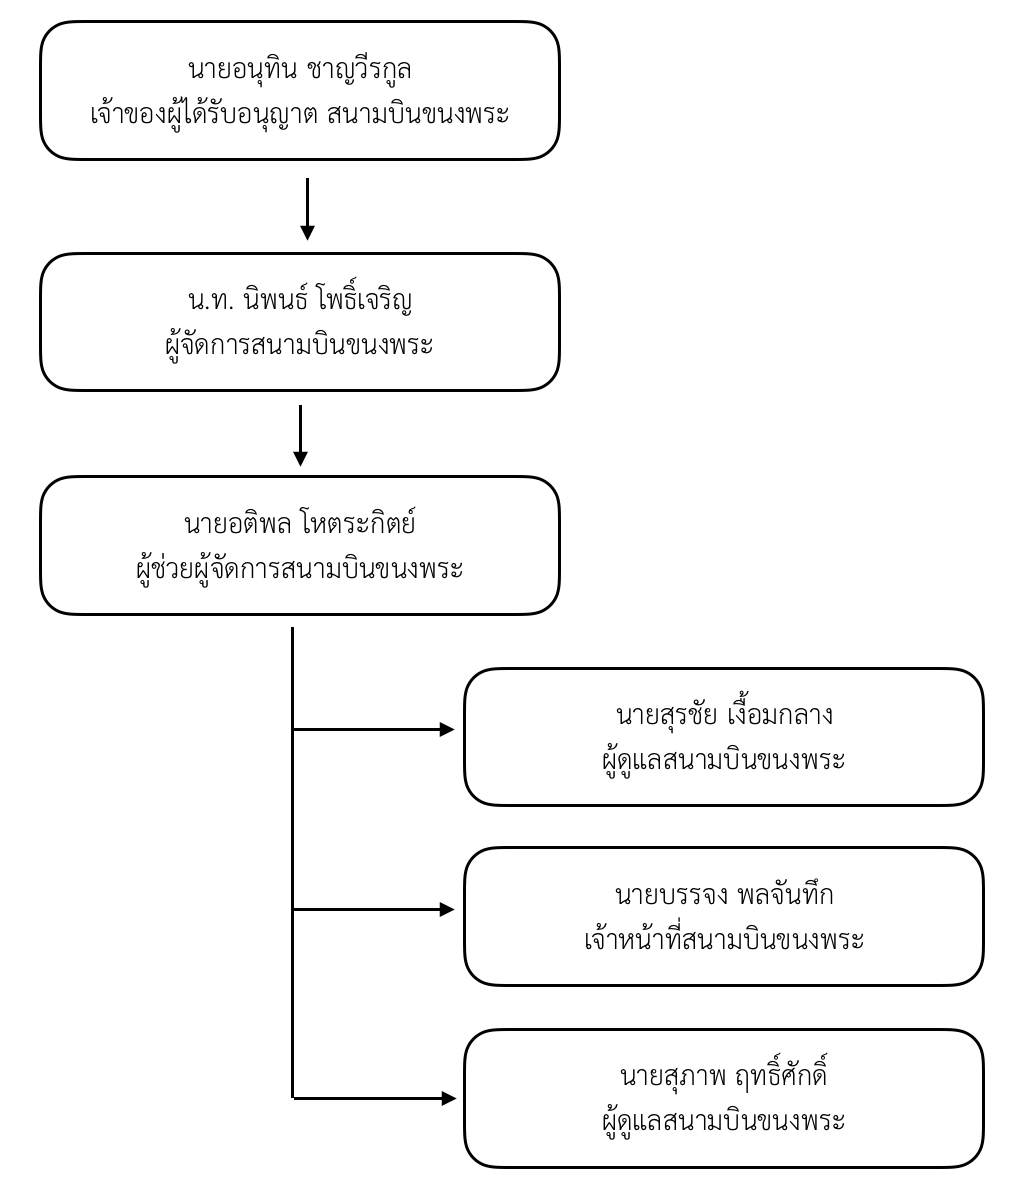
\includegraphics[scale=0.5]{images/KNP_Org_Chart.png}
\caption{แผนผังองค์กรของสนามบินขนงพระ}
\label{แผนผังองค์กรของสนามบินขนงพระ}
\end{center}
\end{figure}

\newpage

\section{บุคลากรรับผิดชอบด้านความปลอดภัยและด้านการรักษาความปลอดภัยของสนามบินขนงพระ}

\begin{table}[ht]
\caption{ผู้รับผิดชอบด้านความปลอดภัยและการรักษาความปลอดภัยของสนามบินขนงพระ}
\begin{center}
\begin{tabular}{clll}
 & & & \\
\textbf{ลำดับ} & \textbf{คำนำหน้า ชื่อ-สกุล} & \textbf{ตำแหน่ง} & \textbf{โทรศัพท์ติดต่อ} \\
1 & น.ท.นิพนธ์ โพธิ์เจริญ & ผู้จัดการสนามบิน & 086 657 1510 \\
2 & นายอติพลโหตระกิตย์ & ผู้ช่วยผู้จัดการสนามบิน & 089 478 0808 \\
3 & นายสุรชัย เงื้อมกลาง & ผู้ดูแลสนามบิน & 097 965 9897 \\
4 & นายบรรจง พลจันทึก & เจ้าหน้าที่สนามบิน & 089 035 9034 \\
5 & นายสุภาพ ฤทธิ์ศักดิ์ & ผู้ดูแลสนามบิน & 085 637 4751 \\ 
\end{tabular}
\end{center}
\label{ผู้รับผิดชอบด้านความปลอดภัยและด้านการรักษาความปลอดภัยของสนามบินขนงพระ}
\end{table}%

\section{คณะกรรมการต่าง ๆ ของสนามบิน (ถ้ามี)}

-ไม่มี-

\section{ข้อมูลอื่นๆ ที่เกี่ยวข้องกับการบริหารสนามบิน}

-ไม่มี-
 			% Chapter 5: Aerodrome Administration
%!TEX TS-program = xelatex
%!TEX encoding = UTF-8 Unicode

\chapter{ผนวก ก.}

\section{ใบอนุญาตที่ขึ้นลงชั่วคราวอากาศยานขนงพระ} \label{ใบอนุญาตที่ขึ้นลงชั่วคราวอากาศยานขนงพระ}

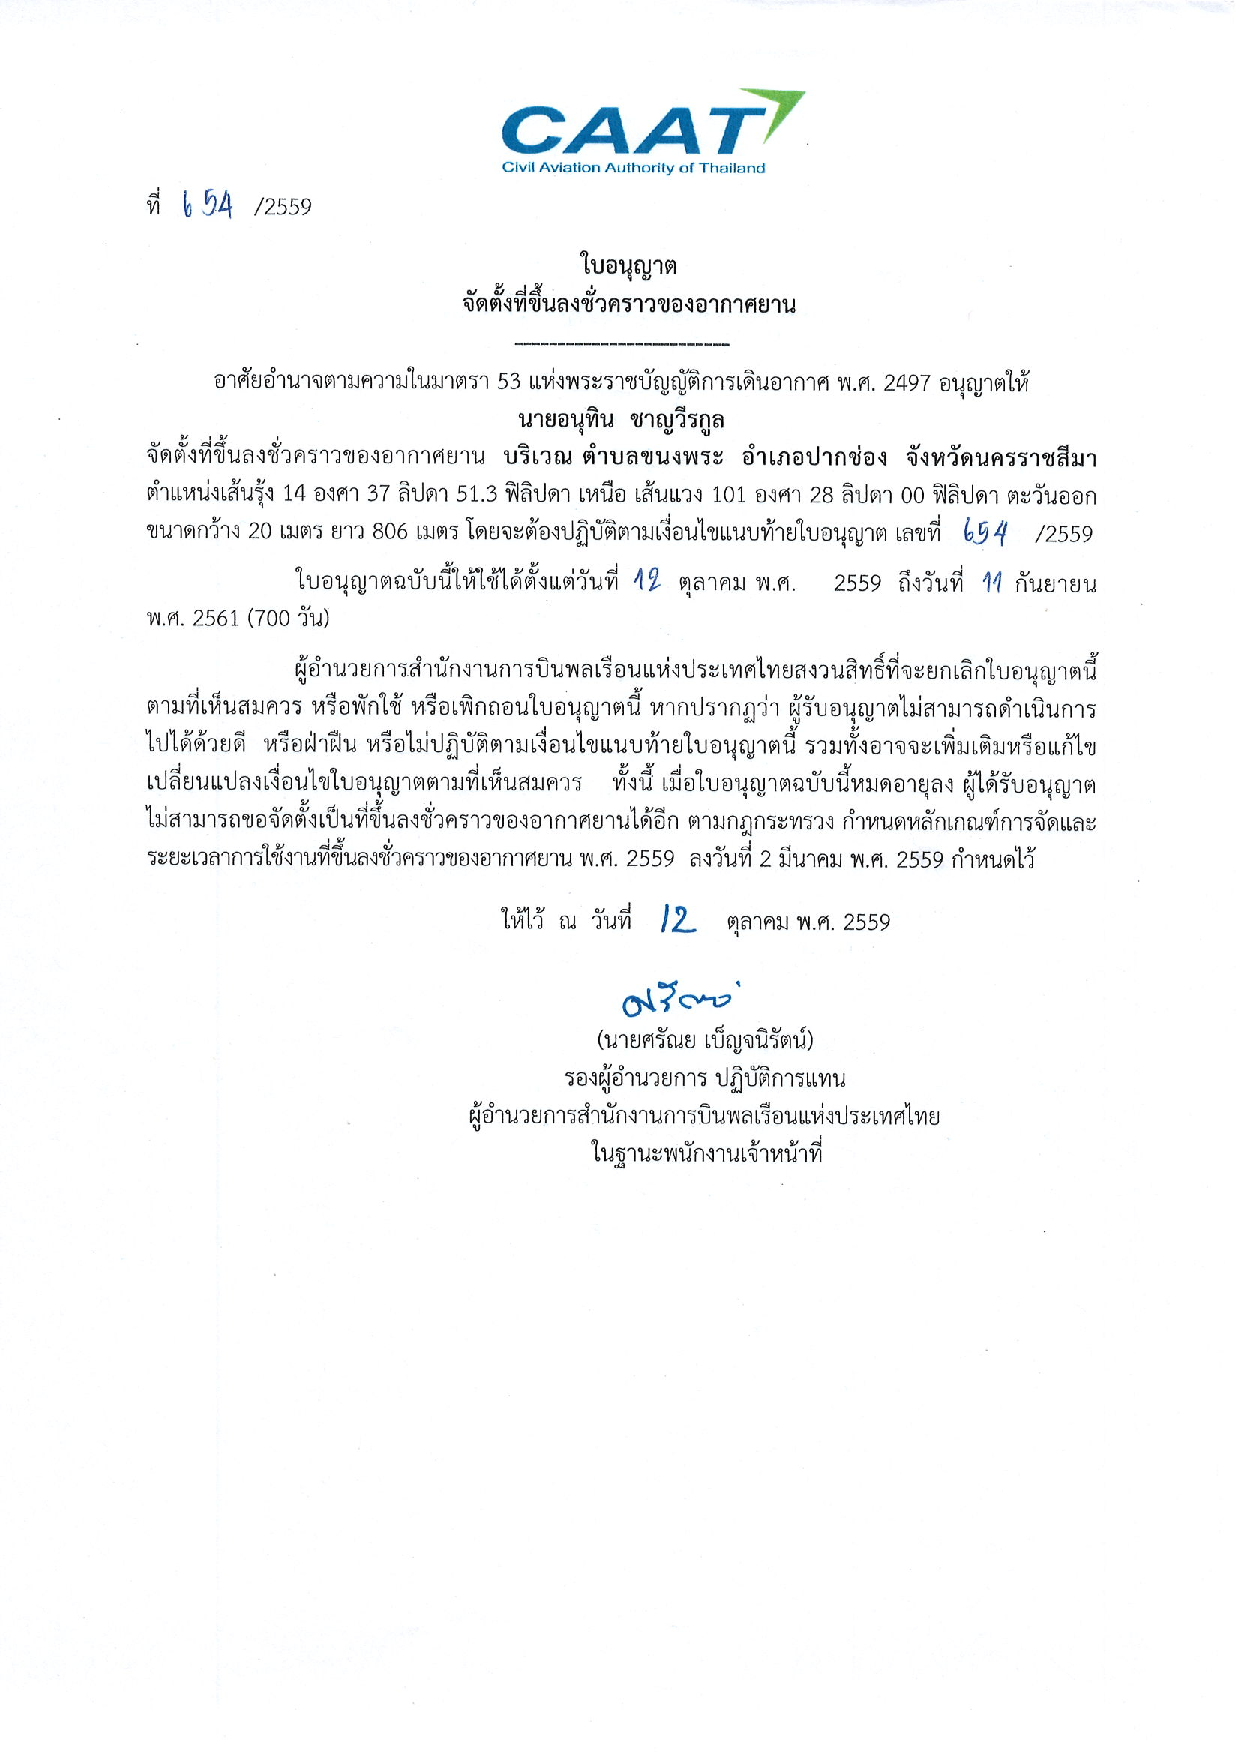
\includepdf[pages=-, pagecommand={}, scale=0.9]{pdf/KNP_Airport_Temp_License_Ending_11-09-2561}	% ผนวก ก. ใบอนุญาตที่ขึ้นลงชั่วคราวอากาศยานขนงพระ
%!TEX TS-program = xelatex
%!TEX encoding = UTF-8 Unicode

\chapter{ผนวก ข. \\
		เอกสารสิทธิ์และหนังสือยินยอมให้ใช้ประโยชน์ที่ดินที่ตั้งสนามบินขนงพระ}
		
\section{เอกสารสิทธิ์และหนังสือยินยอมให้ใช้ประโยชน์ที่ดินจาก บริษัท เจริญคีรี จำกัด} \label{เอกสารสิทธิ์และหนังสือยินยอมให้ใช้ประโยชน์ที่ดินจาก บริษัท เจริญคีรี จำกัด}

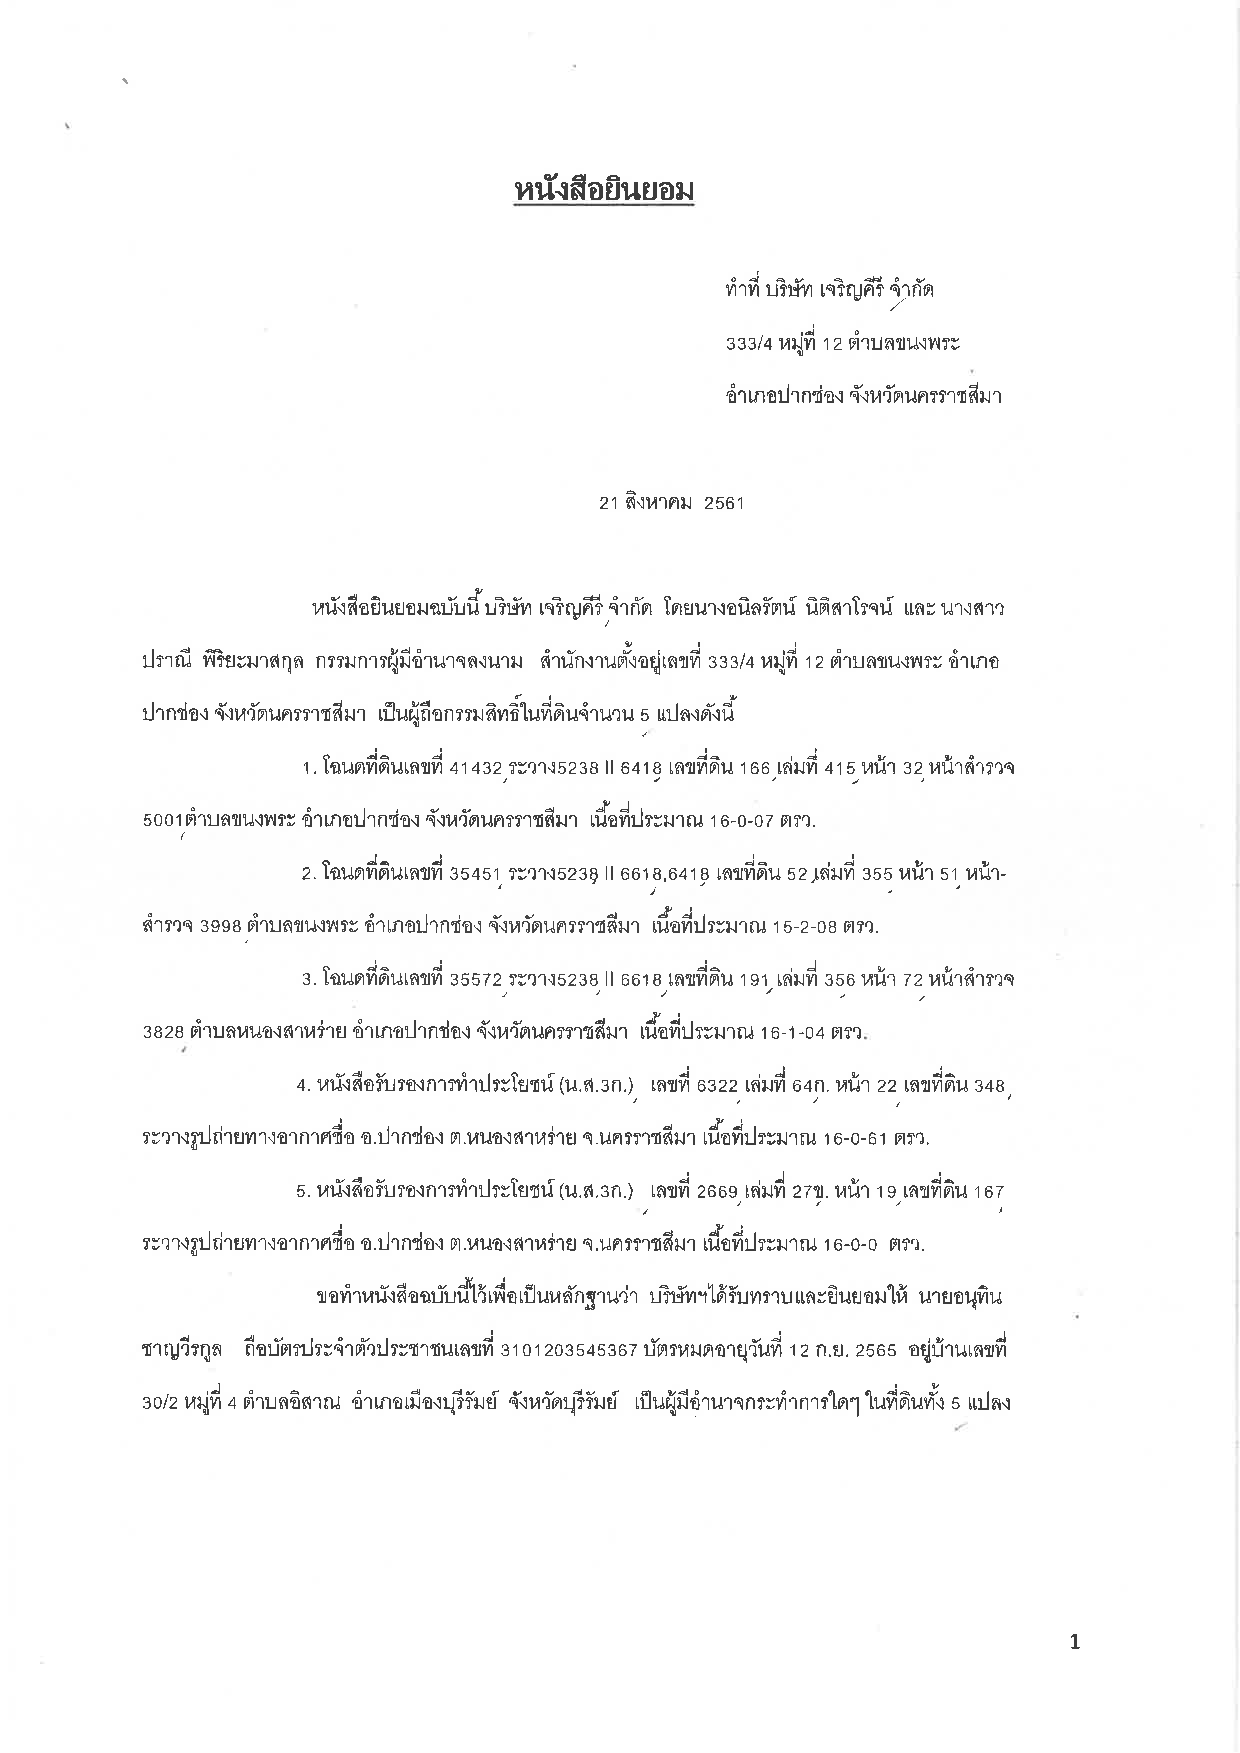
\includepdf[pages=-, pagecommand={}, scale=0.9]{pdf/Land_Deeds_n_Consent_from_CharoenKiriCompany_Part1}
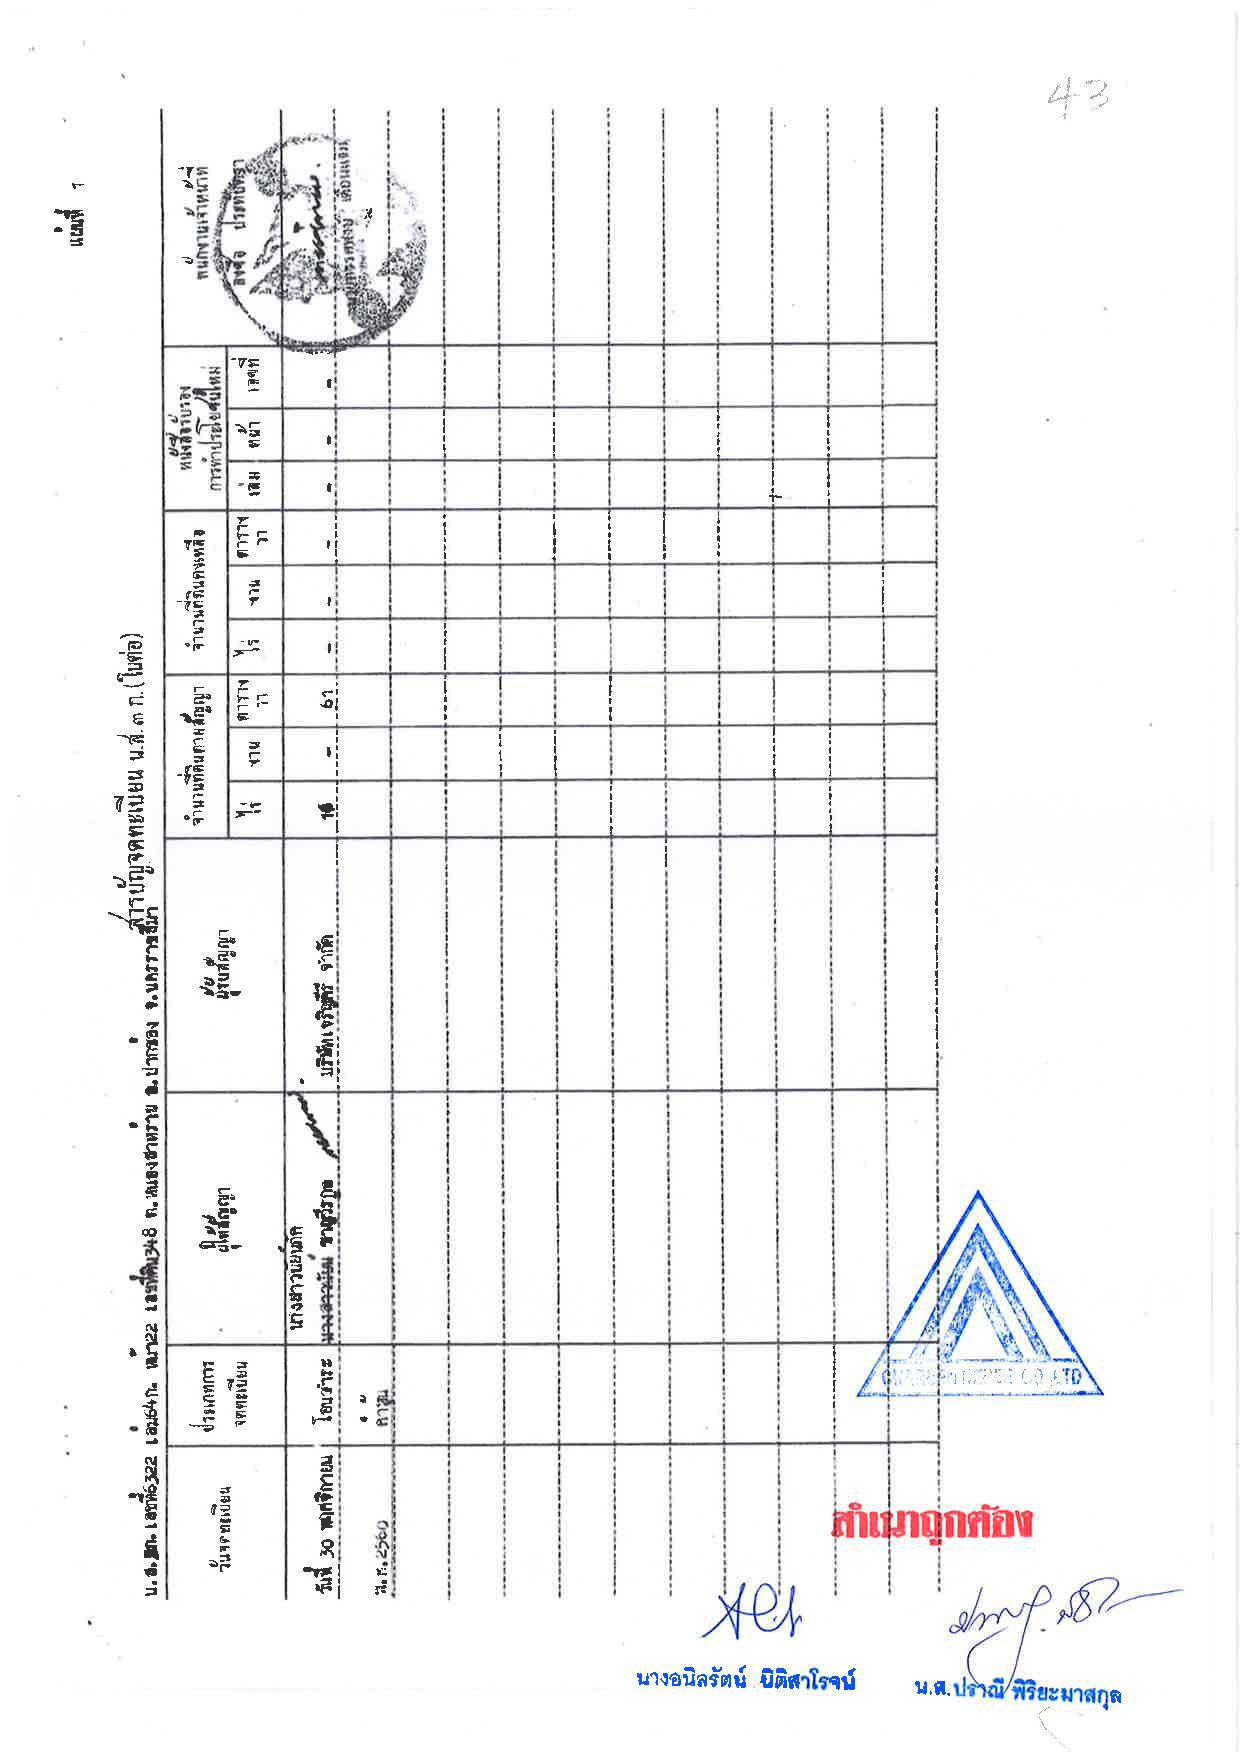
\includepdf[pages=-, pagecommand={}, scale=0.9]{pdf/Land_Deeds_n_Consent_from_CharoenKiriCompany_Part2}

\section{เอกสารสิทธิ์และหนังสือยินยอมให้ใช้ประโยชน์ที่ดินจาก บริษัท กอล์ฟเขาใหญ่ จำกัด} \label{เอกสารสิทธิ์และหนังสือยินยอมให้ใช้ประโยชน์ที่ดินจาก บริษัท กอล์ฟเขาใหญ่ จำกัด}

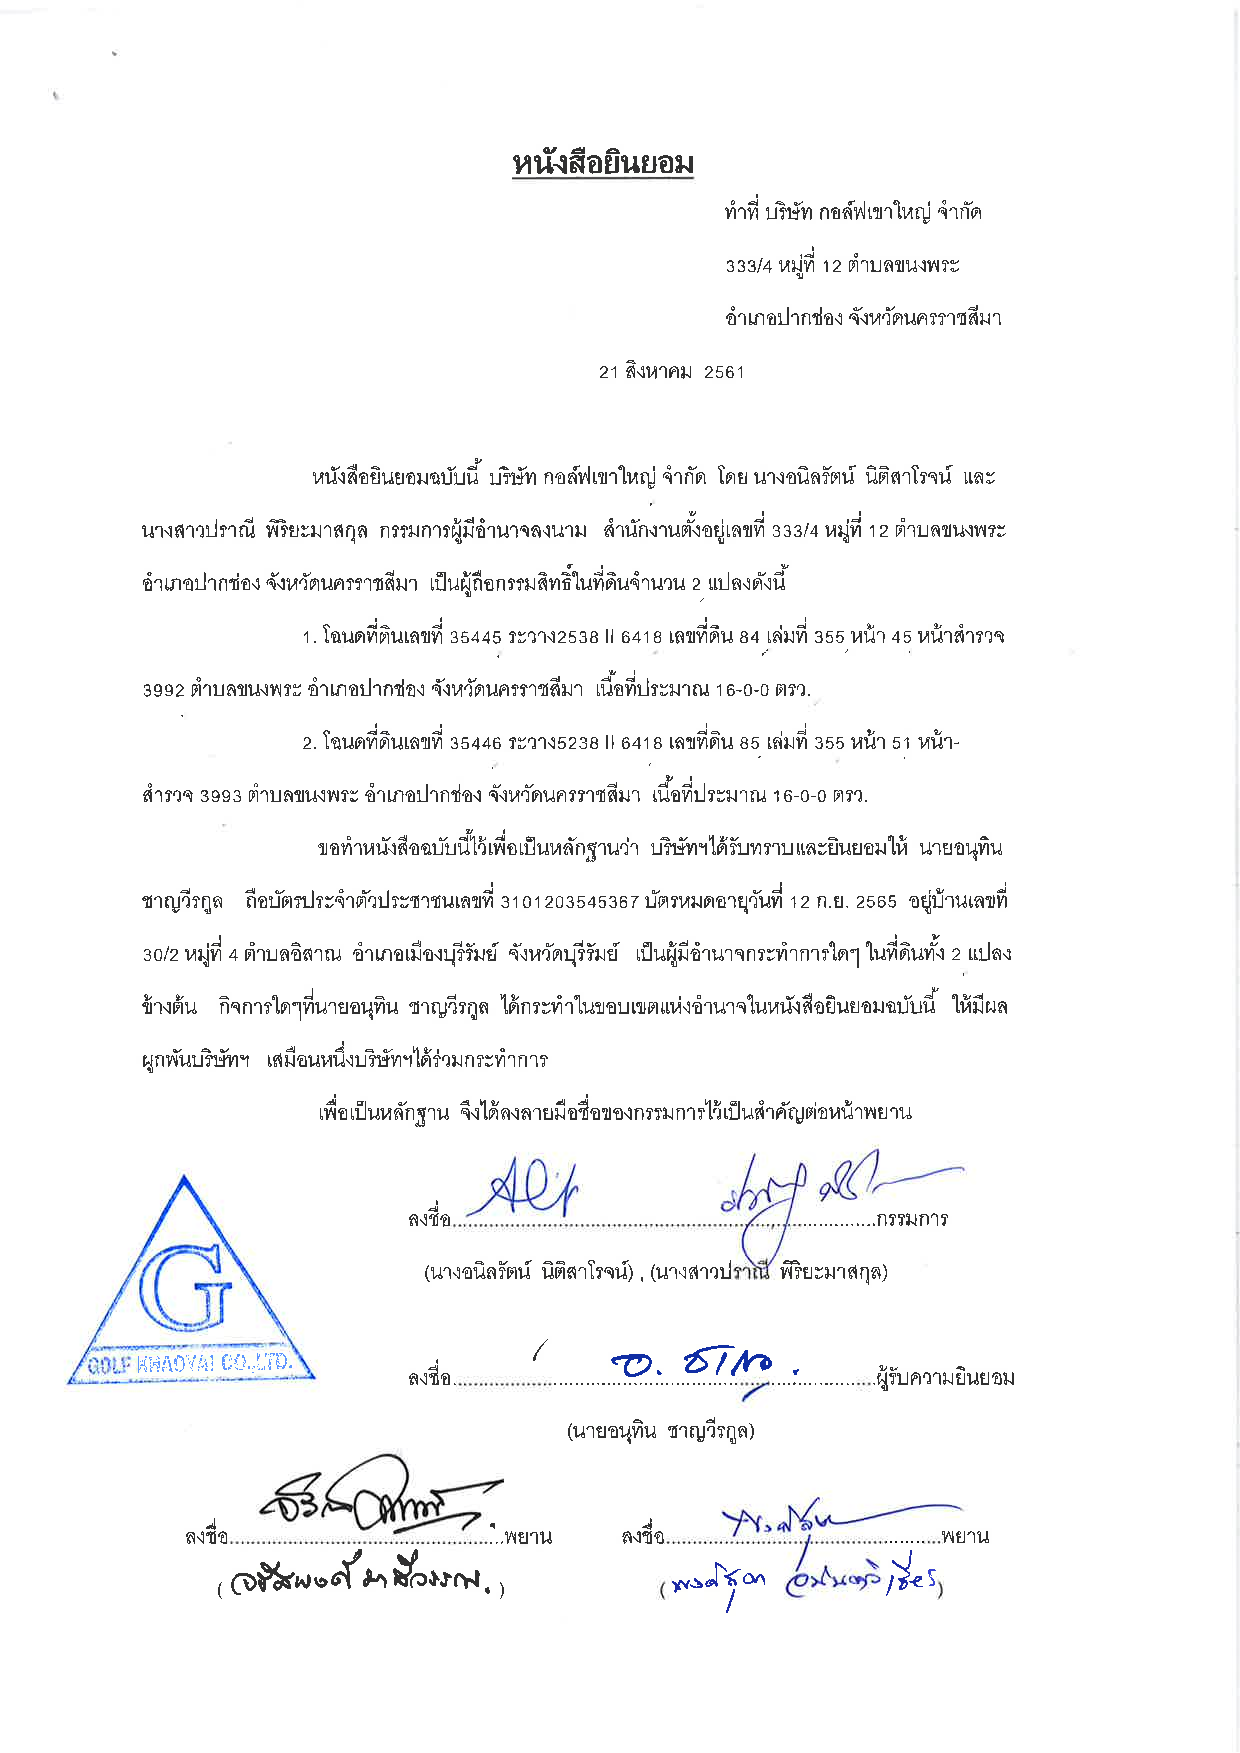
\includepdf[pages=-, pagecommand={}, scale=0.9]{pdf/Land_Deeds_n_Consent_from_GolfKhaoyaiCompany}	% ผนวก ข. เอกสารสิทธิ์และหนังสือยินยอมให้ใช้ประโยชน์ที่ดินที่ตั้งสนามบินขนงพระ
%!TEX TS-program = xelatex
%!TEX encoding = UTF-8 Unicode

\chapter{ผนวก ค.}

\section{รายงานการสำรวจสนามบินส่วนบุคคลขนงพระ} \label{รายงานการสำรวจสนามบินส่วนบุคคลขนงพระ}

\includepdf[pages=2, pagecommand={}, scale=0.85]{pdf/KNP_engineering_survey_report_old}
\includepdf[pages=3-49, pagecommand={}, scale=0.85]{pdf/KNP_survey_report.pdf}

\section{สำเนาใบอนุญาตประกอบวิชาชีพวิศวกรรม ของผู้ควบคุมงานการสำรวจสนามบินขนงพระ}

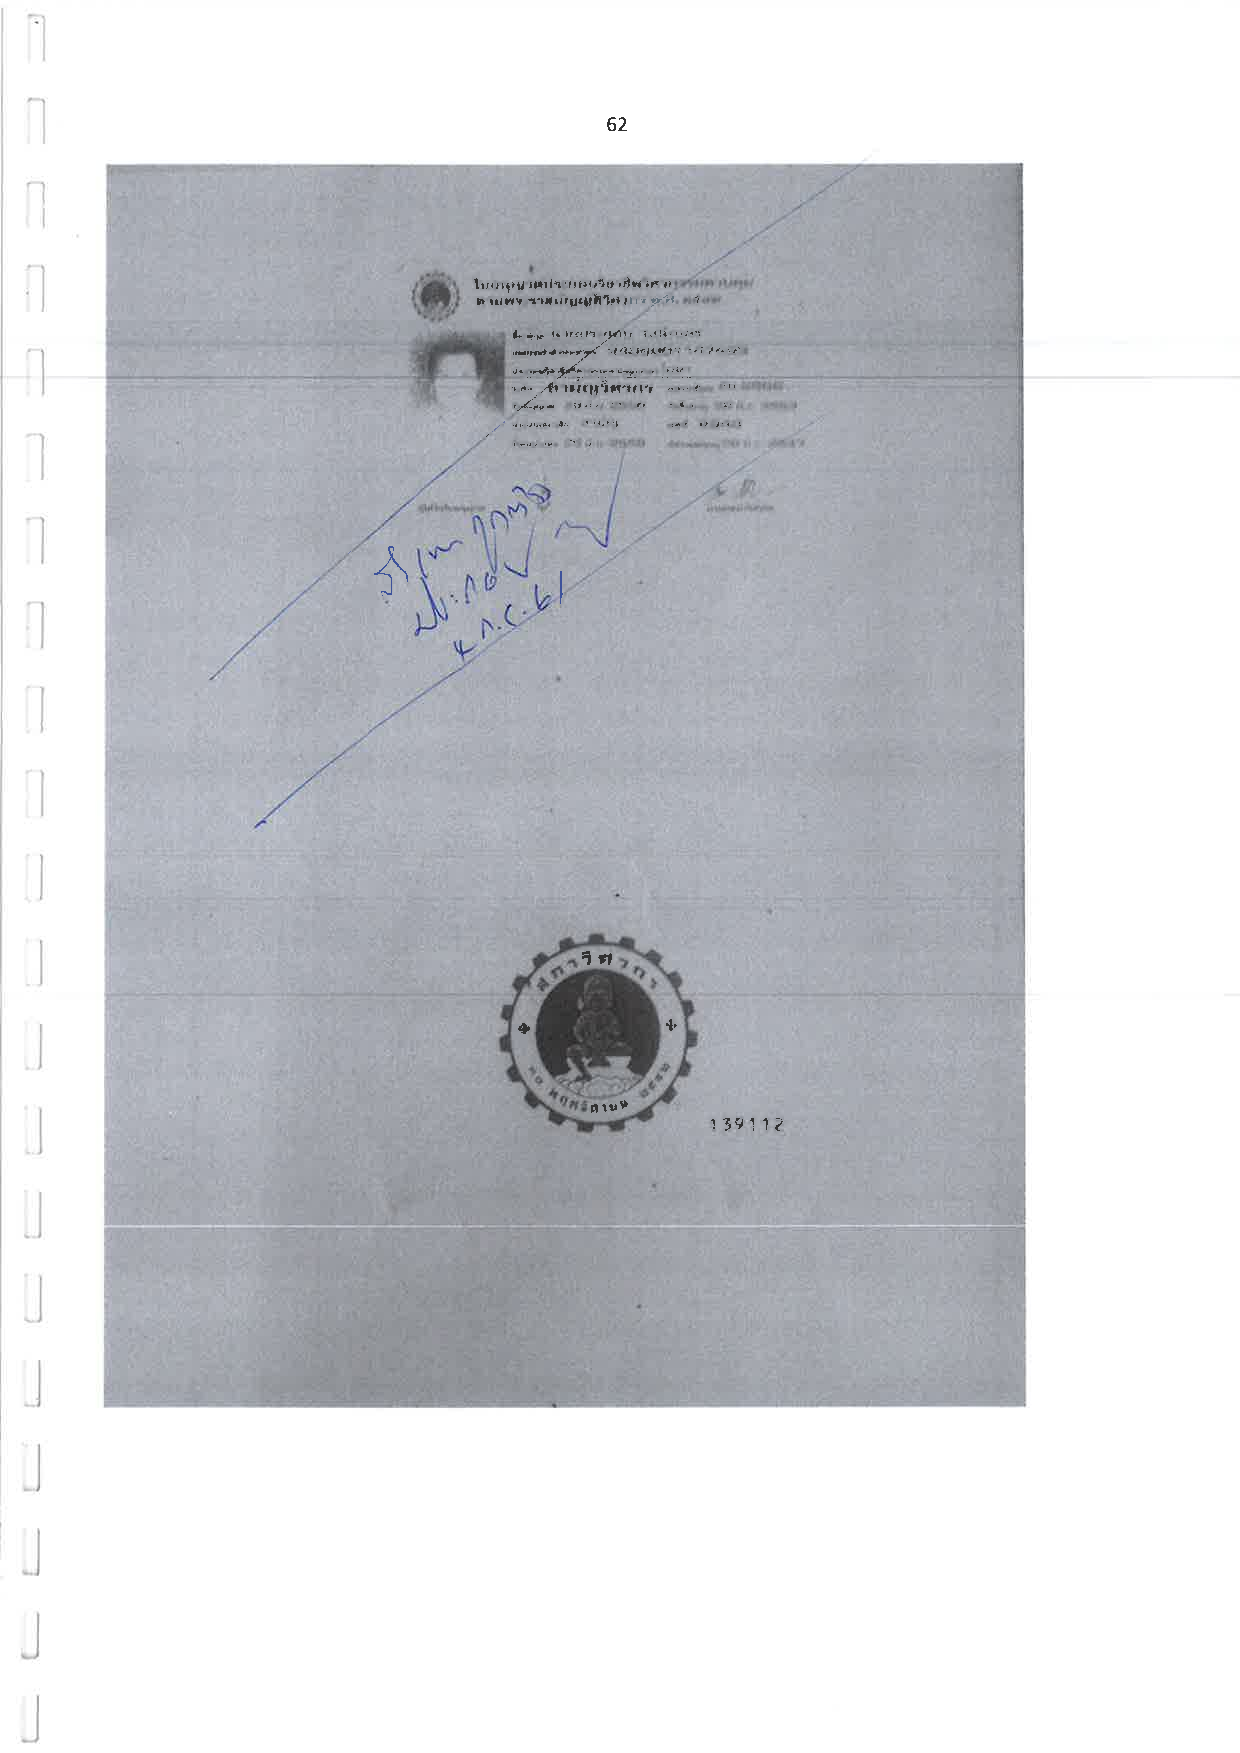
\includepdf[pages=-, pagecommand={}, scale=0.9]{pdf/survey_engeering_license}
	% ผนวก ค. รายงานการสำรวจสนามบินส่วนบุคคลขนงพระ โดยวิศวกร
%!TEX TS-program = xelatex
%!TEX encoding = UTF-8 Unicode

\chapter{ผนวก ง.}

\section{ข้อมูลรายละเอียด Runway ของสนามบินส่วนบุคคลขนงพระ} \label{ข้อมูลรายละเอียด Runway ของสนามบินส่วนบุคคลขนงพระ}

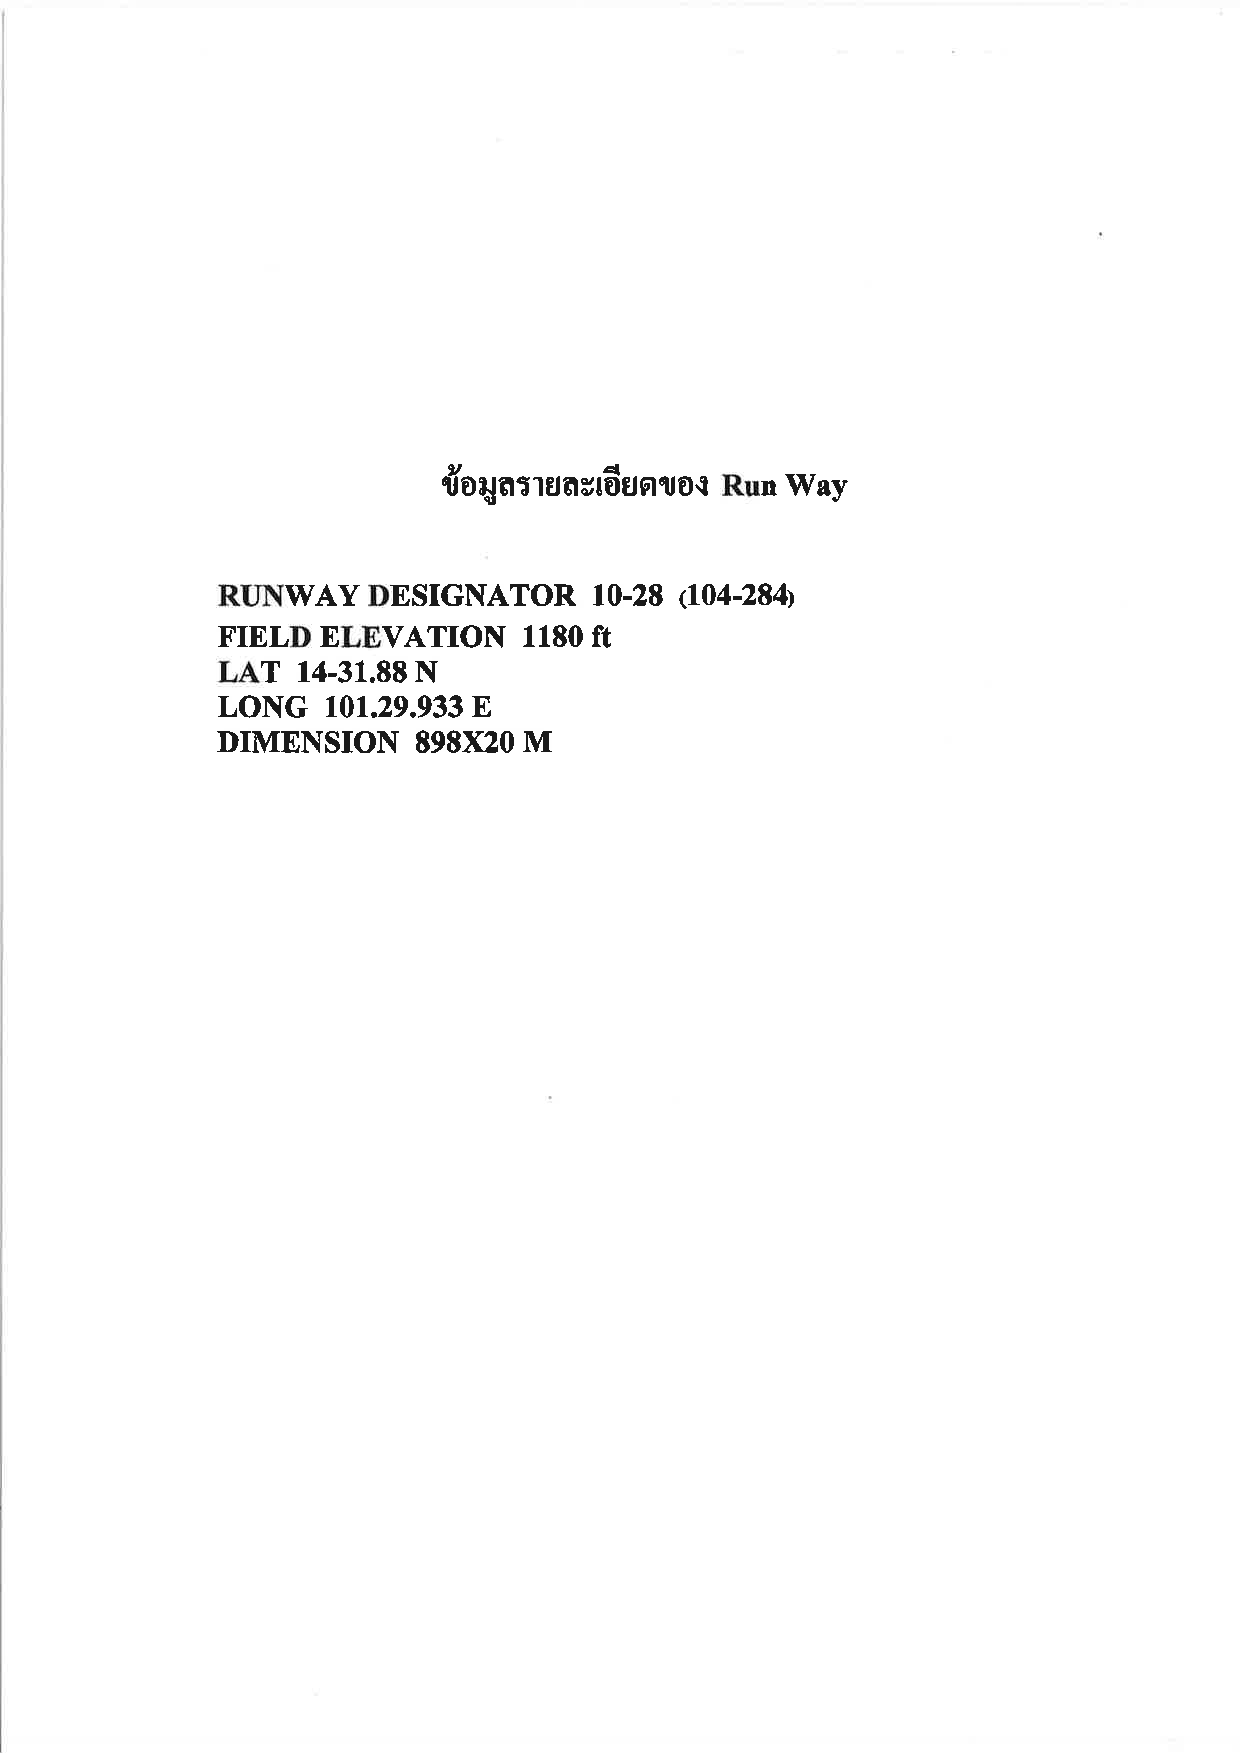
\includepdf[pages=-, pagecommand={}, scale=0.85]{pdf/KanongPhraRunwayDesignDetails}

\section{ข้อมูลรายละเอียดการออกแบบสนามบินส่วนบุคคลขนงพระ} \label{ข้อมูลรายละเอียดการออกแบบสนามบินส่วนบุคคลขนงพระ}

\includepdf[pages=2-, pagecommand={}]{pdf/KanongPhraRunwayDesignDiagram}	% ผนวก ง. ข้อมูลรายละเอียดของ Runway ขนงพระ
%!TEX TS-program = xelatex
%!TEX encoding = UTF-8 Unicode

\chapter{ผนวก จ. }

\section{แบบฟอร์ม KNP-Form-01 รายงานการตรวจพินิจพื้นที่เคลื่อนไหว}

\begin{landscape}
\begin{table}[h!]
%\caption{}
\begin{center}
\begin{tabular}{|c|c|c|c|c|c|c|c|c|c|c|c|c|c|c|c|c|c|}
\hline
\multirow{3}{*}{วัน/เดือน/ปี} & \multirow{3}{*}{เวลาตรวจ}  & \multicolumn{2}{c|}{\multirow{3}{*}{สภาพทางวิ่ง}} &  \multicolumn{2}{c|}{\multirow{3}{*}{FOD}} &  \multicolumn{2}{c|}{ถุงลม} &  \multicolumn{2}{c|}{\multirow{3}{*}{สัตว์ในเขต}} &  \multicolumn{2}{c|}{\multirow{3}{*}{จุดน้ำขัง}} &  \multicolumn{2}{c|}{การบุกรุก} &  \multicolumn{2}{c|}{สิ่งปลูกสร้าง} & หมายเหตุ  & ลงชื่อ \\ % Heading row
 & & \multicolumn{2}{c|}{} & \multicolumn{2}{c|}{} & \multicolumn{2}{c|}{สีหมายเลขทางวิ่ง} & \multicolumn{2}{c|}{} & \multicolumn{2}{c|}{} & \multicolumn{2}{c|}{เขตพื้นที่} & \multicolumn{2}{c|}{อุปสรรค} & ระบุสิ่งไม่ปกติ & ผู้ตรวจพื้นที่ \\
 & & \multicolumn{2}{c|}{} & \multicolumn{2}{c|}{} & \multicolumn{2}{c|}{} & \multicolumn{2}{c|}{} & \multicolumn{2}{c|}{} & \multicolumn{2}{c|}{} & \multicolumn{2}{c|}{ต่อการบิน} & สิ่งที่พบและการแก้ไข &  \\
\hline
 &  & ปกติ & ไม่ปกติ & มี & ไม่มี & ปกติ & ไม่ปกติ & พบ & ไม่พบ & มี & ไม่มี & มี & ไม่มี & มี & ไม่มี & & \\
 \hline
 & & & & & & & & & & & & & & & & &  \\
 \hline
&  & & & & & & & &  & &  & & & & & & \\
\hline
& &  & & & & & & & & & & & & & & & \\
\hline
 & & & & & & & & & & & & & & & & & \\
\hline
& & & & & & & & & & & & & & & & & \\
\hline
\end{tabular}
\end{center}
%\label{}
\end{table}%
\textbf{การกรอก}
\begin{enumerate}
\item ระบุ วัน เวลา
\item ระบุ โดย check ปกติหรือไม่ปกติ    มีหรือไม่มี  พบหรือไม่พบ  หากไม่ปกติ     มีหรือพบ ให้ระบุในช่อง หมายเหตุ ว่า ไม่ปกติอย่างไร พบอะไร หรือ มีอะไร และ ได้แก้ไขไปอย่างไร
\item ลงชื่อ ทุกวัน  เมื่อครบเดือน ให้นำเสนอผู้ควบคุมสนามบิน
\item หากช่องกรอกไม่เพียงพอ ให้เขียนรายงานสิ่งที่ตรวจพบ และสิ่งที่ต้องแก้ไข แนบเพิ่มเติมได้ 
\end{enumerate} %

\vskip 10pt
ลงลายมือ ………………………………..........................
\vskip 10pt
ชื่อ-สกุล ................................................................. %
\end{landscape}
	% ผนวก จ. แบบฟอร์มรายงานการตรวจสนามบิน
%!TEX TS-program = xelatex
%!TEX encoding = UTF-8 Unicode

\chapter{ผนวก ฉ.}\label{ผนวก ฉ.}

\section{แบบฟอร์ม Bird Strike Report Form ของ สำนักงานการบินพลเรือนแห่งประเทศไทย}\label{แบบฟอร์ม Bird Strike Report Form ของ สำนักงานการบินพลเรือนแห่งประเทศไทย}

\begin{figure}[ht]
\begin{center}
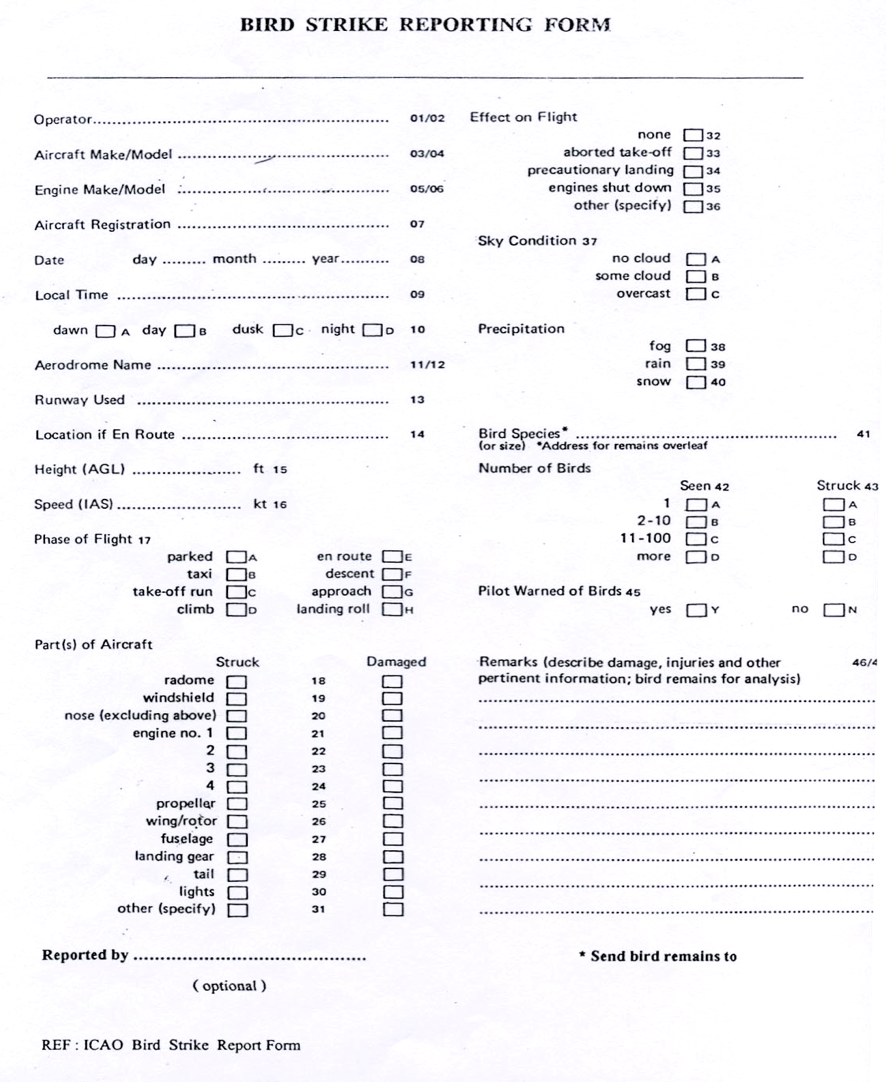
\includegraphics[width=\linewidth]{images/Bird_Strike_Report_Form.png}
\caption{Bird Strike Reporting Form}
\label{Bird Strike Reporting Form}
\end{center}
\end{figure}	% ผนวก ฉ. CAAT Bird Strike Report Form

\end{document} 